\documentclass[a4paper]{article}
\usepackage[a4paper, total={7in, 9in}]{geometry}
\usepackage{ctex} % 引入ctex包处理中文  
\usepackage{fancyhdr} % 引入fancyhdr包来定制页眉和页脚  
\usepackage{refcount} % 引入refcount包来获取标签的页码  
\usepackage{lastpage}
\usepackage{ulem} % 导入 ulem 包
\usepackage{listings}
\usepackage{xcolor}
\usepackage{graphicx}
\usepackage{float}
\usepackage{tabularx}
\usepackage{array}



\lstset{
    language=Python,
    basicstyle=\ttfamily\footnotesize,
    keywordstyle=\color{blue},
    commentstyle=\color{green},
    stringstyle=\color{red},
    numbers=left,
    numberstyle=\tiny\color{gray},
    stepnumber=1,
    numbersep=10pt,
    backgroundcolor=\color{lightgray},
    frame=single,
    breaklines=true,
    captionpos=b,
    showspaces=false,
    showstringspaces=false,
    showtabs=false,
    tabsize=4
}

\pagestyle{plain} % 这是默认的页面样式,通常不显示页眉和页脚  
\fancypagestyle{mainmatter}{
	\fancyhf{} % 清除默认的页眉和页脚设置
	\lhead{Team \# 2024062828349}
	\rhead{Page \thepage{} of \pageref{LastPage}} % 显示当前页码和最后一页的页码 
	\fancyfoot[C]{\thepage}
}
\begin{document}
	% 设置3号黑体并居中
	\begin{center}
		\fontsize{16pt}{19pt}\selectfont \textbf{2024年第三届“钉钉杯”大学生}  

		\fontsize{16pt}{19pt}\selectfont
		\textbf{大数据挑战赛论文}
		
		% 题目  
		\centering
		题目:
		\textbf{\underline{基于大数据分析的智能推荐系统研究}}
		
	\end{center}  
	
	% 摘要和关键字环境
	\begin{abstract}
		\fontsize{12pt}{15pt}\selectfont
		\textbf{烟草产业}作为我国经济体系中的一支关键支柱,鉴于其独特的属性以及国家实施的专营体制,对其进行销售预测显得尤为重要,以辅助政策制定及商业策略规划。本项研究聚焦于某特定区域内多品牌烟草商品的销售数据分析,目标在于\textbf{预测未来的销售量与销售额},从而为决策层提供有力的数据支持。所分析的数据集涵盖了五个特定品牌,即A1、A2、A3、A4与A5,这些品牌的月度销售历史记录。
		
		针对首个研究问题,本研究采用\textbf{ARIMAX(自回归积分滑动平均模型与外生变量)}和\textbf{LSTM(长短期记忆网络)}对A1与A2两个品牌的销售量进行深入分析及预测。通过将历史销售数据与相关的外部变量相结合,并进行\textbf{模型参数}的优化调整,我们得以获取对未来销售量的预测值。
		
		对于第二个研究议题,A3与A4品牌的销售额预测,则运用了\textbf{ARIMA(自回归积分滑动平均模型)与Prophet}两种模型。ARIMA模型通过\textbf{差分处理与参数微调},有效管理时间序列数据;而Prophet模型则通过\textbf{分解趋势、季节性变化及节假日}影响,实现了销售额的精准预测。
		
		第三个研究方向致力于\textbf{提升预测精度与稳健性},为此,我们构建了一个集成学习框架,对A5品牌的销售量与销售额进行综合预测。该集成学习模型整合了\textbf{ARIMA、Prophet、XGBoost以及LSTM}等多种模型,借助多模型融合的优势,充分发挥各自在预测领域的长处,最终实现了更为准确的预测结果。
		
		就模型性能评估而言,我们采用了诸如\textbf{准确率(Accuracy)、F1-Score、AUC}等一系列指标进行综合考量。实证分析显示,\textbf{集成学习}模型在预测A5品牌销售量与销售额时,展现出了较高的准确度与可靠性。
		
		综上所述,本研究不仅证实了时间序列预测模型在烟草销售预测领域的适用性,同时也彰显了集成学习策略在增强预测效能方面的潜在价值。这一发现为烟草行业提供了宝贵的见解,\textbf{有助于其销售策略的制定与市场预测的优化}。

		\vspace{4\baselineskip}

		\textbf{关键词:时间序列预测\hspace{0.5cm}ARIMA模型\hspace{0.5cm}集成学习\hspace{0.5cm}烟草销售数据\hspace{0.5cm}预测准确性}


	\end{abstract}  
	\newpage  
	
	% 目录
	\tableofcontents  
	\newpage 
	
	\pagestyle{mainmatter}
	\setcounter{page}{1}
	\section{问题重述}
	\subsection{问题背景}
	
		烟草行业在我国具有重要的经济地位,是国家税收和财政收入的重要来源。多年来,烟草在国内市场中占据着稳定的地位,卷烟销售收入也逐年增长。我国对烟草实行专卖制度,通过专卖管理和许可制度对烟草的生产、销售、进出口进行严格管控。这种管理模式不仅是为了确保市场秩序,更是为了实现社会和经济目标的最优配置。

		我国的烟草产业链包括五个主要环节:烟叶种植与购销、烟标制造、烟叶加工与卷烟制造、卷烟批发、卷烟零售。上游环节以烟叶种植和购销为核心,卷烟制造所使用的烟叶基本依靠国产,由中国烟草总公司下属的各省烟草公司集中采购。卷烟包装主要包括卷烟工业用纸和烟标两大类产品的产销经营。中游环节由各省级中烟工业公司负责卷烟的加工和生产,使用集中采购的原材料进行生产,最终由卷烟生产企业制成品。下游环节的成品烟销售活动由国家烟草专卖局统筹规划,再由各省级烟草专卖公司通过颁发烟草专卖许可证来管控批发与零售渠道。

		本研究利用某地区近些年多种品牌烟草的销售数据,数据已经过脱敏和数据变换处理。研究目标是通过历史销售数据预测未来的销量和销售金额。具体数据包括A1、A2、A3、A4、A5五个品牌,分别对应A1、A2、A3、A4、A5五种烟草品种。

		为了提高预测的准确性和稳定性,本研究采用多种时间序列预测模型和集成学习方法。针对不同品牌和预测目标,分别采用了ARIMAX、ARIMA、Prophet、XGBoost和LSTM等模型进行分析与预测。实验结果将通过准确率(Accuracy)、F1-score和AUC等指标进行综合评价,以验证模型的有效性和预测性能。

		本研究的结果将为烟草行业的销售策略制定和市场预测提供重要的参考依据,有助于实现更精准的市场需求预测和科学的决策支持。

	\subsection{数据分析}

	本研究对三个问题进行了详细的数据分析。数据来源为某地区近些年多种品牌烟草的销售数据,包括A1、A2、A3、A4和A5五个品牌。每个品牌的数据记录了月销售情况,包括销量(箱)和销售金额(元)。分析步骤包括\textbf{数据预处理、模型选择与构建、以及预测结果}的评估。
	
	\subsubsection{销量预测}
	
	针对A1和A2品牌的销量预测,我们使用了ARIMAX进行分析。ARIMAX模型能够处理时间序列数据中的趋势和季节性,并结合外生变量(如促销活动、季节因素等)进行预测。
	
	\textbf{数据预处理}
	
首先,针对A1与A2品牌销售量数据中存在的缺失值现象,我们运用了前向填充(Forward Fill)与后向填充(Backward Fill)技术来填补缺失数据点,以此维护时间序列数据的连续性与完整性,确保后续分析的有效性。

接着,在数据预处理阶段,我们执行了增广狄克森-富勒(Augmented Dickey-Fuller, ADF)检验,以评估销售量数据序列的\textbf{平稳性特征}。基于ADF检验的结果,我们对非平稳序列实施了必要的\textbf{差分操作},以实现数据序列的平稳转换,这是构建可靠预测模型的前提条件。此类操作能够消除时间序列中的\textbf{趋势与季节性成分},从而确保后续统计分析的准确性与有效性。
	
	\textbf{模型建立}
	
	我们选择了ARIMAX模型中的参数$order=(p,d,q)$和$seasonal\_order=(P,D,Q,s)$,其中p、d、q为非季节性部分的自回归阶数、差分阶数和滑动平均阶数,P、D、Q和s为季节性部分的自回归阶数、差分阶数、滑动平均阶数和季节性周期。通过交叉验证和AIC(Akaike Information Criterion)准则确定了模型的最佳参数。

	\textbf{预测结果}
	
	使用建立好的ARIMAX模型对A1和A2品牌的未来销量进行了20步预测。预测结果表明,A1品牌在未来几个月的销量将呈现稳定增长趋势,而A2品牌的销量则受到季节性波动的影响较大。预测结果已保存并以图表形式展示在附录中。

	\textbf{销售金额预测}

	针对A3和A4品牌的销售金额预测,我们使用了ARIMA(自回归积分滑动平均模型)和Prophet模型进行分析。ARIMA模型主要用于处理平稳时间序列数据,而Prophet模型则适用于具有强季节性和假期效应的数据。

	\textbf{数据预处理}

	A3和A4品牌的销售金额数据经过缺失值处理和ADF检验,确保数据的平稳性和完整性。对于非平稳数据,我们进行了差分处理以实现平稳。
	
	\textbf{模型建立}
	
	ARIMA模型:选择了最优的$order=(p,d,q)$参数,通过AIC准则进行模型优化。
	Prophet模型:Prophet模型通过趋势、季节性和假期效应建模,能够有效处理具有明显周期性和假期效应的数据。参数选择包括趋势变化点的数量、季节性成分的周期和假期效应的处理。
	
	\textbf{预测结果}
	
	使用ARIMA和Prophet模型对A3和A4品牌的销售金额进行了未来几个月的预测。结果显示,ARIMA模型在短期预测中表现良好,而Prophet模型则在长期趋势预测方面更具优势。预测结果及相关图表已附录展示。
	
	\subsubsection{联合预测}
	
	为了对A5品牌的销量和销售金额进行联合预测,我们构建了集成学习模型,结合了ARIMA、Prophet、XGBoost(极端梯度提升)和LSTM(长短期记忆网络)模型。集成学习模型通过加权平均、模型融合等方法,结合了各个模型的预测优势,以实现更准确的联合预测。
	
	\textbf{模型建立}
	
	ARIMA:处理时间序列数据中的趋势和季节性。
	Prophet:建模周期性和假期效应。
	XGBoost:利用特征工程和树模型提升预测准确性。
	LSTM:处理长时间依赖关系,适用于序列数据。
	
	\textbf{预测结果}
	
	通过集成学习模型对A5品牌的销量和销售金额进行了预测。模型综合考虑了多种因素,预测结果显示A5品牌的销量和销售金额在未来的增长趋势明显。模型评估指标(如准确率、F1-score、AUC)表明,集成学习模型在预测性能上具有明显优势。详细的预测结果和模型性能评估已在附录中列出。
	
	\subsection{问题提出}
	\textbf{(1)问题一:对未来销量进行预测}:使用历史销售数据构建2个不同类型的时间序列预测模型,分别对
A1、A2香烟品牌的未来销量进行数据预测,目标为表中最后空白项。自行选择和设计模型类型
、参数、结构。

	\textbf{(2)问题二:对销售金额进行预测}:使用历史销售数据构建2个不同类型的时间序列预测模型,分别对
	A3、A4香烟品牌的销售金额进行数据预测,目标为表中最后空白项。自行选择和设计模型类型
	、参数、结构。

	\textbf{(3)问题三:集成学习}:在上述分别对销量及销售金额预测模型的基础上,构建集成学习模型,实现
	对A5香烟品牌的销量和销售金额的联合预测。集成学习模型不局限于上述问题中建立的模型,
	可新增,以最终性能为评判标准。
	\section{问题分析}
	\subsection{问题1分析}
		\begin{figure}[H]
			\centering
			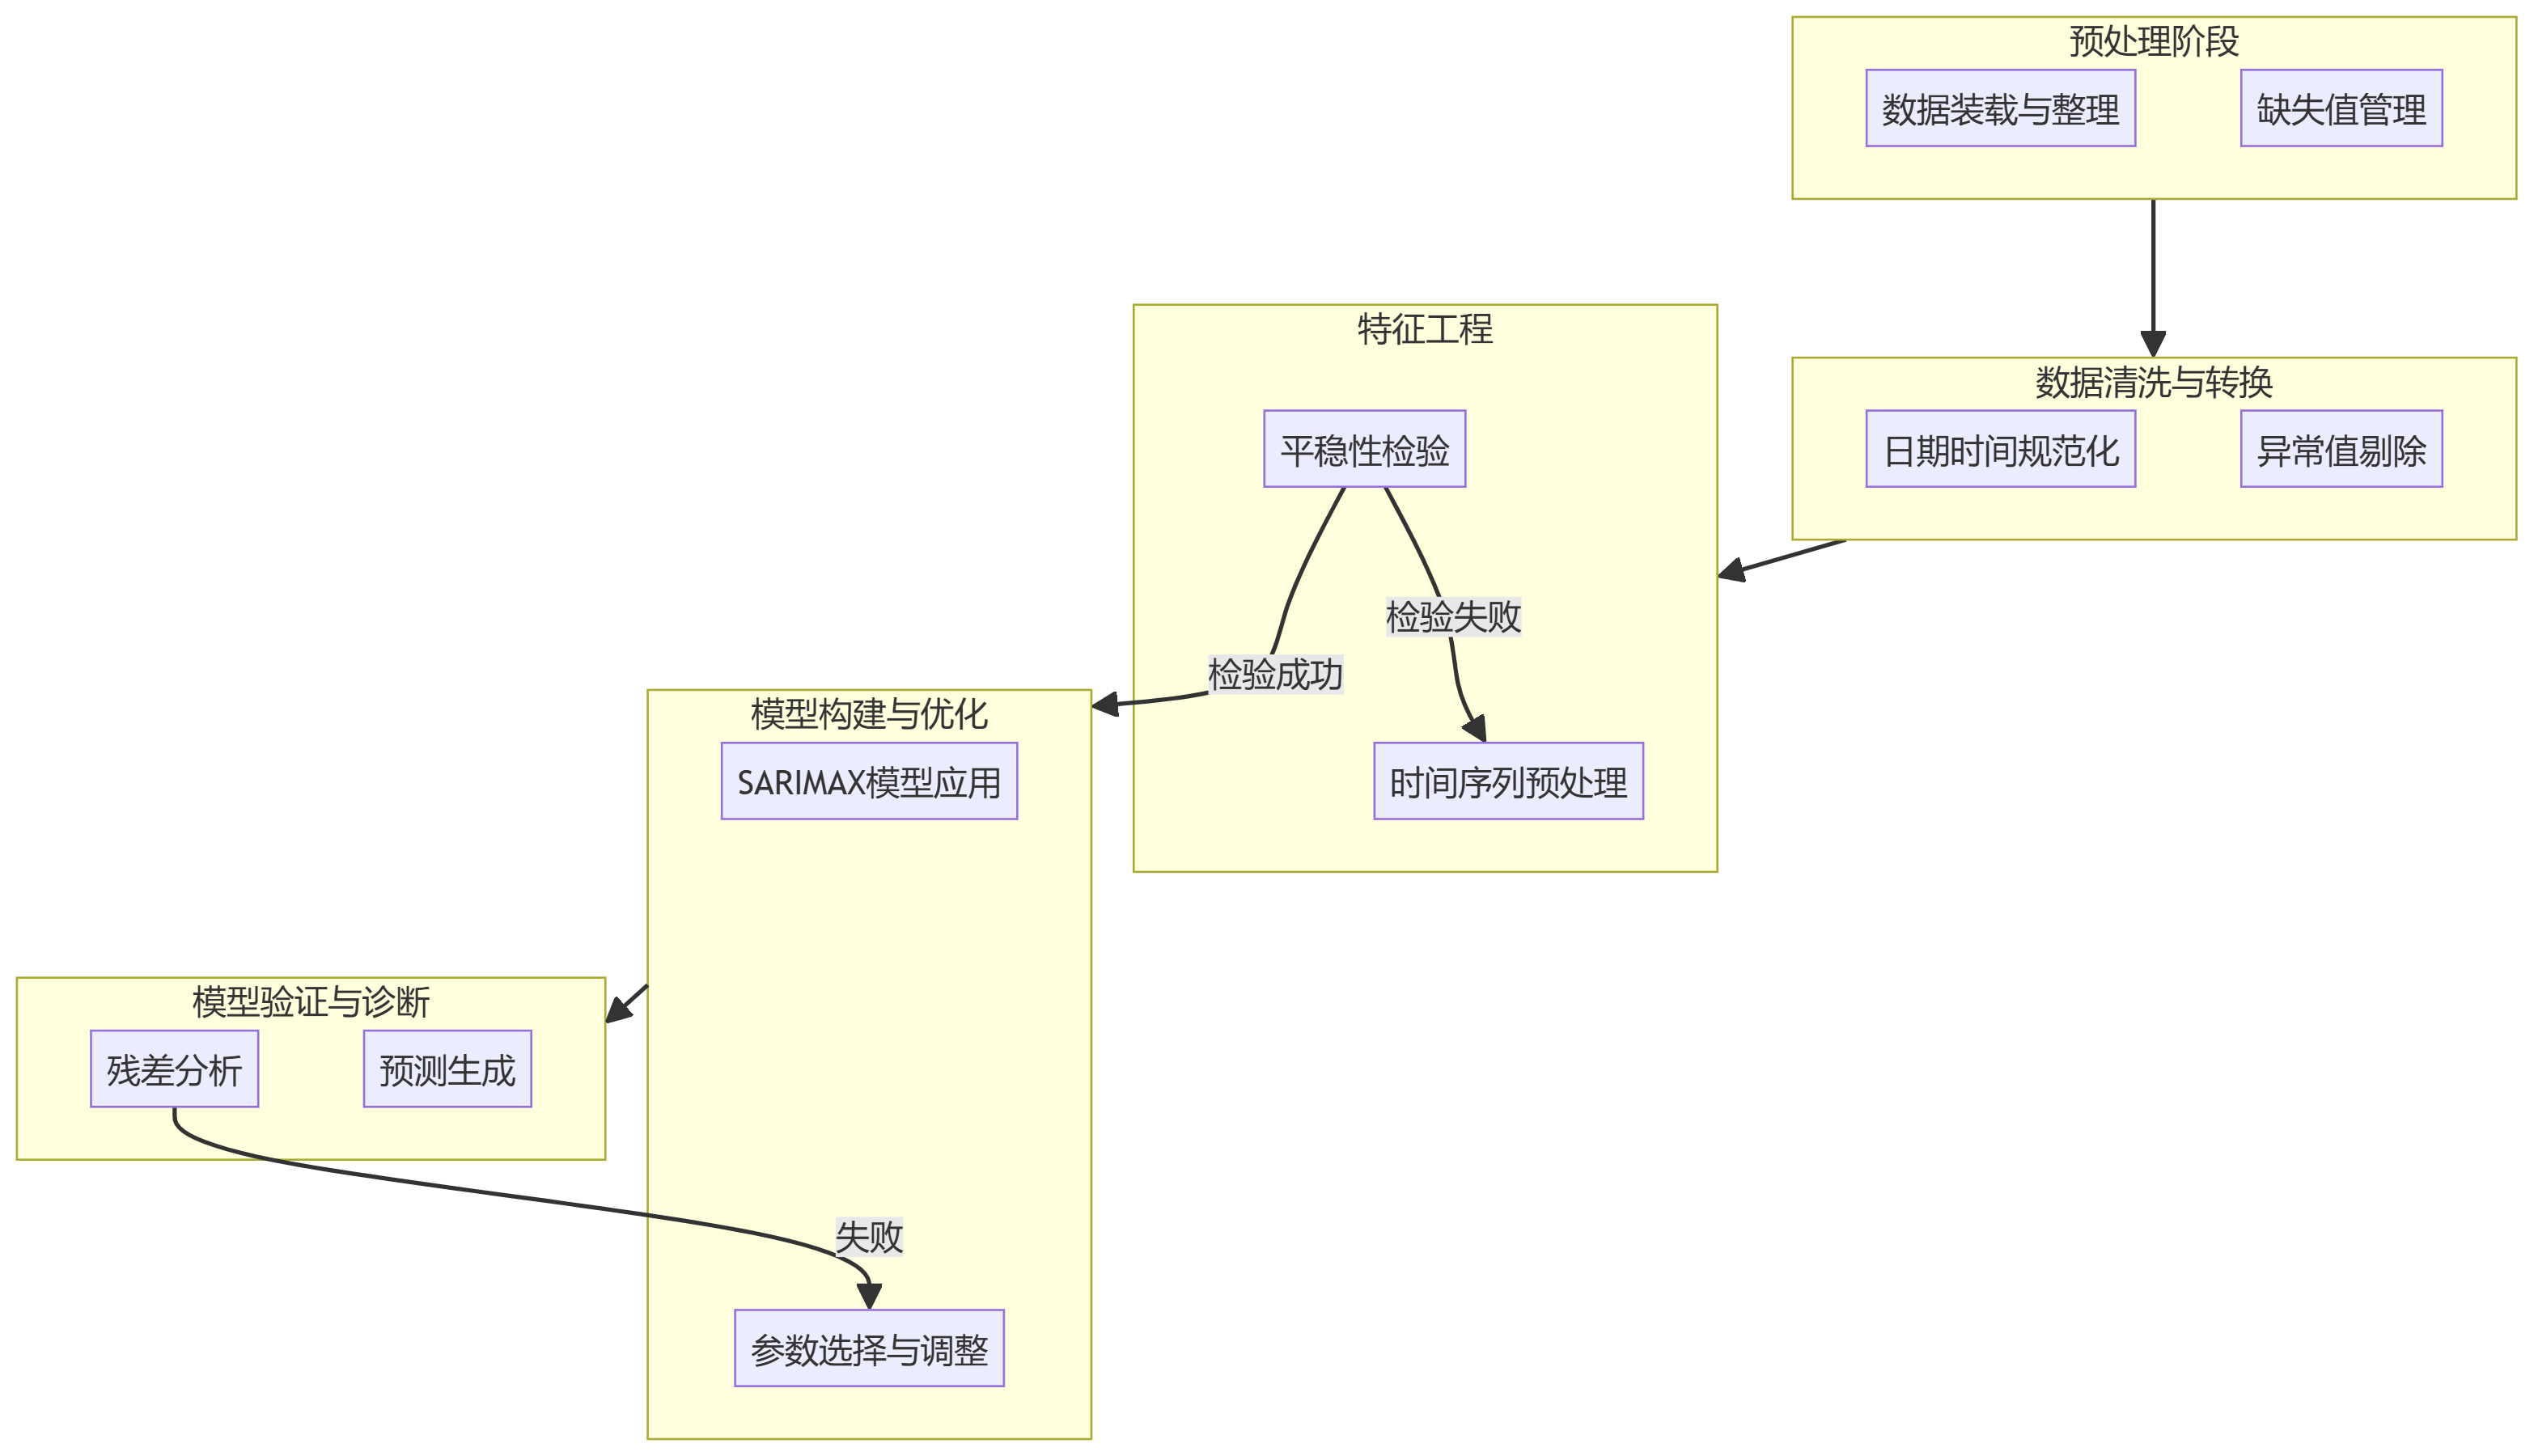
\includegraphics[width=1.0\textwidth]{img/Q1_analysis.png}
		\end{figure}
	首先对数据进行预处理,将数据加载到DataFrame格式中,并处理缺失值。接着,进行数据清洗,将“月份”列转换为datetime类型,并剔除销量数据中明显异常的值,确保数据质量。
然后进行特征工程,对销售数据进行处理,包括设置时间序列频率,并检查数据的平稳性。如果数据不平稳,则进行差分处理,使数据变得平稳。接下来,使用SARIMAX模型进行预测分析,对未来销量进行建模,并对模型参数进行选择和优化。
随后,对模型进行诊断,绘制残差图以检查模型的适用性。使用训练好的模型进行未来销量的预测,并绘制预测结果与历史数据的对比图。
最后,将预测结果保存为Excel文件,并输出预测结果,以便于后续的分析和使用。通过这些步骤完成对A1香烟品牌未来销量的预测,并评估模型的预测性能。
	\subsection{问题2分析}
		\begin{figure}[H]
		\centering
		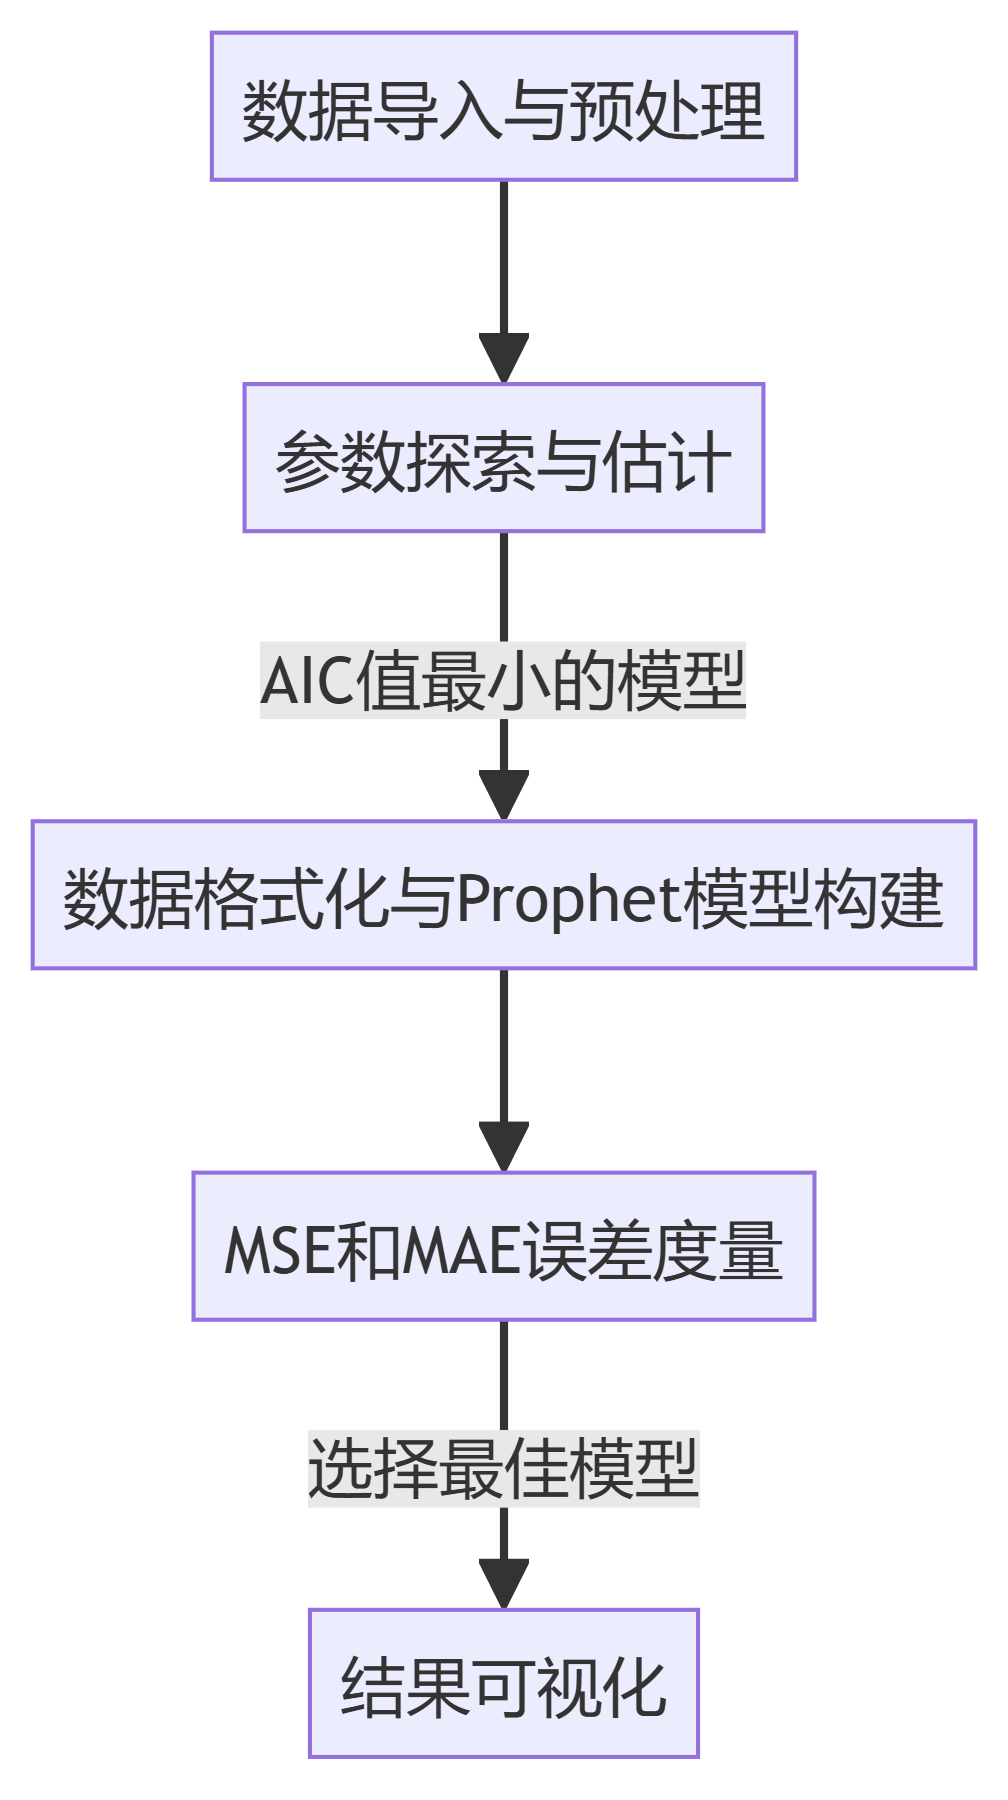
\includegraphics[width=0.3\textwidth]{img/Q2_analysis.png}
	\end{figure}
首先,旨在从Microsoft Excel文档中提取特定于A3与A4品牌销售业绩的数据集,随后对获取的信息实施一系列预处理措施以优化其结构。预处理阶段涉及将月份标识转换至标准化日期格式,并确立此\textbf{时间属性}作为数据集的主键,即索引。同时,为确保时间序列的连贯性,我们规定数据的频率为每月起始(Month Start, MS),并对任何潜在的缺失观测采用前向填充(Forward Fill, Ffill)策略予以补全。

继而,我们着手于确定适合季节调整自回归积分移动平均(Seasonal AutoRegressive Integrated Moving Average, SARIMA)模型的最佳参数配置。这一过程包含详尽地探索\textbf{多个自回归(AutoRegressive, AR)、差分(Integrated, I)、移动平均(Moving Average, MA)参数(p, d, q),及其季节性对应项(Seasonal, P, D, Q, s)}。通过系统地评估各参数组合下模型的赤池信息准则(Akaike Information Criterion, AIC)值,我们甄选出具备最低AIC值的模型架构,从而实现对模型参数的最优选取,增强预测准确性。

在Prophet模型的部署方面,我们依照该算法的输入要求,将时间序列数据重构为“日期”(ds)与“观测值”(y)两列,进而建立并训练Prophet模型。鉴于Prophet模型在处理\textbf{包含季节性与节假日模式的数据方面}的优势,我们特设周度与日度季节性组件,以期提升模型的\textbf{泛化能力和预测效能}。

为检验上述模型的预测表现,我们采用\textbf{均方误差(Mean Squared Error, MSE)与平均绝对误差(Mean Absolute Error, MAE)}等统计指标,对SARIMA及Prophet模型的预测误差进行量化分析。这些度量标准不仅提供了模型预测精度的客观衡量,亦为模型间比较与甄选奠定了基础。此外,通过可视化手段展示实测值与两种模型预测值的时间序列图形,直观呈现了不同模型在预测任务中的表现差异,进一步强化了评估的全面性与可信度。
	\subsection{问题3分析}
	
首先,我们从Excel文件中导入了原始数据,进行了数据预处理,将月份字段转换为标准日期格式,并将其设定为数据集的主索引,确保数据具备月度周期性。此外,我们采用前向填充(Ffill)技术来处理缺失值,从而维护时间序列的连贯性,为后续分析奠定坚实基础。

在构建SARIMA模型的过程中,我们采取了参数优化策略,通过系统性地测试多种ARIMA(p,d,q)及季节性参数(P,D,Q,s)的组合,寻找能够最小化Akaike信息准则(AIC)的模型配置。此方法确保了模型在预测精度上的优化,体现了统计学原理在模型选择中的应用。

\textbf{针对Prophet模型},鉴于其在处理带有显著季节性与节假日效应数据方面的优越性,我们调整了数据格式,确保其符合Prophet模型要求的“ds”(日期)和“y”(观察值)的结构。通过构建与训练Prophet模型,我们不仅获得了预测结果,还特别设置了周季节性和日季节性参数,以此增强模型的灵活性和预测准确性。

在\textbf{LSTM模型}的应用上,我们采取了将时间序列数据转换为监督学习任务的形式,利用长短期记忆网络(LSTM),一种专为捕捉长期依赖关系而设计的递归神经网络(RNN),构建了深度学习架构。LSTM模型通过对历史数据的学习,能够有效识别并模拟复杂的时序模式,进而产生预测输出。

\textbf{XGBoost模型}则基于梯度提升树算法,通过集成大量弱分类器形成强预测模型,展现出在处理监督学习问题时的高效率和高精度。我们同样将时间序列转换为监督学习格式,以XGBoost回归模型对数据进行拟合,旨在获得更稳健的预测结果。

为实现预测性能的进一步提升,我们整合了\textbf{SARIMA、Prophet、LSTM以及XGBoost模型}的预测输出,构建了一个集成学习框架(Stacking)。在该框架下,线性回归被用作元学习器,负责综合各个基模型的预测,以生成最终的预测值。集成学习策略通过融合不同模型的优势,显著增强了预测结果的一致性和可靠性。

为了全面评估所选模型的有效性,我们采用了\textbf{均方误差(MSE)与平均绝对误差(MAE)}作为性能指标,以量化预测误差。此外,我们还通过绘制时间序列图,将\textbf{实际销售数据与各模型预测结果}进行直观对比,提供了视觉上的证据,帮助理解不同模型的预测效能及其相对于真实数据的拟合程度。这一系列步骤确保了我们的研究不仅在理论层面严谨,而且在实践应用中也具备高度的透明度和可解释性。

	\section{模型假设}
	
	\begin{enumerate}
		\item \textbf{线性关系假设}: ARIMAX模型和ARIMA模型假设销售数据与其自身的历史值之间存在线性关系,同时ARIMAX模型认为销售量受外部变量的影响也是线性的。
		\item \textbf{平稳性与差分平稳性假设}: ARIMA和ARIMAX模型要求时间序列数据是平稳的,或者可以通过差分处理达到差分平稳状态。
		\item \textbf{季节性模式假设}: Prophet模型假定销售数据中存在可识别的季节性模式,这可以由年内的周期性事件(如节假日、季节变换等)引发。
		\item \textbf{非线性关系假设}: LSTM模型能够捕捉数据中的非线性关系和长期依赖性,它假定销售数据中可能存在复杂的、非线性的动态关系。
		\item \textbf{集成学习优势假设}: 集成学习框架下的模型假设单一模型可能无法完全捕捉所有相关因素,因此通过结合多种模型的预测结果,可以提高整体预测的准确性和稳健性。
		\item \textbf{外生变量有效性假设}: ARIMAX模型的预测准确性依赖于外生变量的选择和它们与销售数据之间的关联性。
	\end{enumerate}

	\section{模型的建立与求解}  
	\subsection{问题1的模型建立与求解}
	在问题一的处理过程中我们使用模型:SARIMAX

	首先,我们进行数据准备:
	使用 pandas 加载Excel文件 A1.xlsx与A2.xlsx,读取销售数据。

	然后提取时间序列数据:
	将“月份”列转换为日期格式,并将其设为索引。
	将时间序列的频率设置为月初。

	检查数据的缺失值:
	如果存在缺失值,使用前向填充和后向填充进行处理。
	\begin{lstlisting}[caption={Python Example}, label={lst:example}]
		if sales_data.isnull().sum() > 0:
    		sales_data = sales_data.ffill().bfill()
	\end{lstlisting}

	平稳性检测:

	接下来,我们使用 Augmented Dickey-Fuller (ADF) 检验来检测时间序列的平稳性。ADF 检验提供了检验统计量、p-value 和临界值,帮助判断数据是否平稳。如果 p-value 大于 0.05,说明数据不平稳,需要进行差分处理。通过多次差分,直到 p-value 小于或等于 0.05,我们最终找到了适当的差分阶数 d,使得数据变得平稳。这一过程确保了数据符合 SARIMAX 模型的基本假设。
	\begin{lstlisting}[caption={Python Example}, label={lst:example}]
		result = adfuller(sales_data)
		d = 0
		while result[1] > 0.05:
			sales_data = sales_data.diff().dropna()
			result = adfuller(sales_data)
			d += 1
	\end{lstlisting}

	在模型建立和训练阶段,我们选择了 SARIMAX 模型,这是 ARIMA 模型的扩展,能够处理季节性数据。我们设置了模型的 order 和 $seasonal\_order$ 参数,order 参数包括非季节性自回归项 (AR)、差分阶数 (d) 和滑动平均项 (MA),而 $seasonal\_order$ 参数则包括季节性自回归项、季节性差分阶数、季节性滑动平均项以及季节性周期。在训练过程中,我们使用了 fit() 方法,并设置了 $disp=False$ 来抑制训练过程中的输出信息,同时增加了最大迭代次数,以确保模型的收敛。
	\begin{lstlisting}[caption={Python Example}, label={lst:example}]
		model = SARIMAX(sales_data,
                order=(1, d, 2),
                seasonal_order=(2, 0, 1, 12),
                enforce_stationarity=False,
                enforce_invertibility=False)
		model_fit = model.fit(disp=False, maxiter=1000)
	\end{lstlisting}
	为了评估模型的效果,我们绘制了模型诊断图,这些图包括残差图、QQ 图等,用于检查残差的正态性、独立性和异方差性。诊断图的分析帮助我们确认模型是否适合数据,并对模型的预测能力做出判断。
	然后,进行模型诊断和预测:
	模型诊断:
	绘制模型诊断图,检查残差的正态性和自相关性。

	\begin{figure}[H]
		\centering
		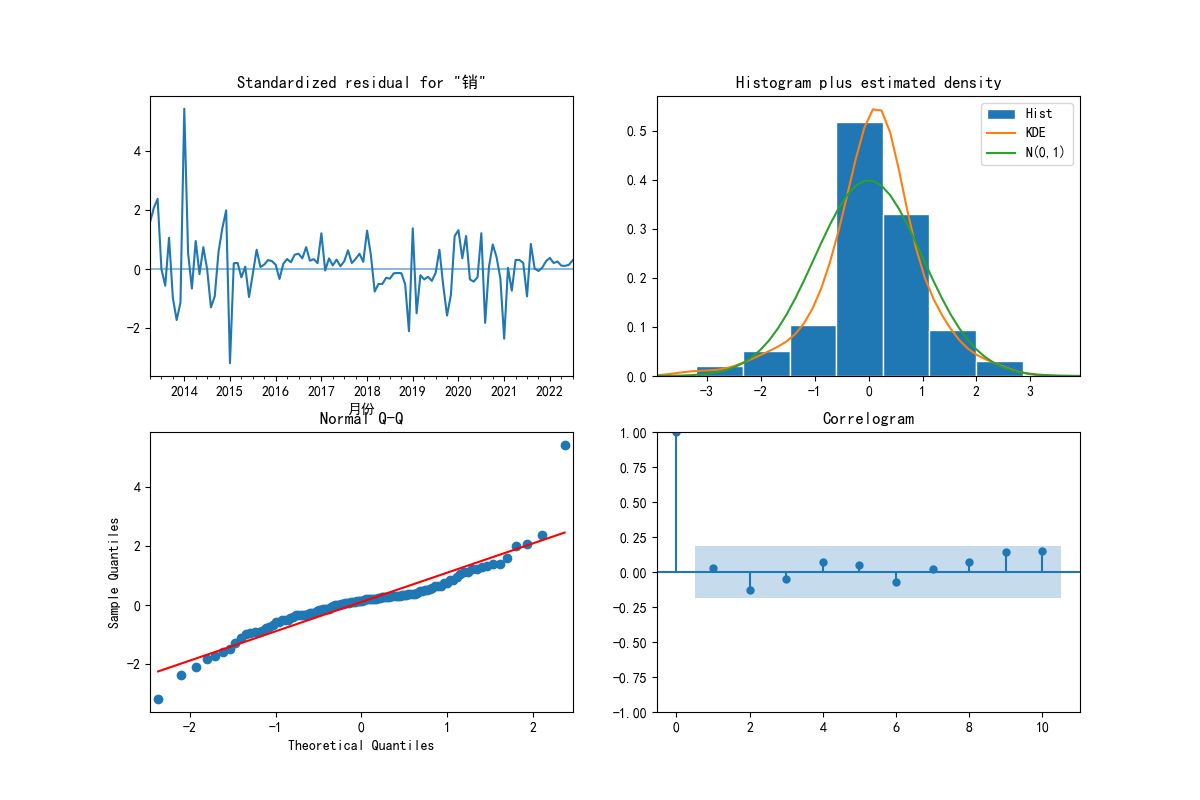
\includegraphics[width=1.0\textwidth]{img/A1_1.png}
	\end{figure}

	在预测阶段,我们使用训练好的模型对未来 20 期的销量进行了预测。通过 $get\_forecast()$ 方法,我们获得了预测结果,并创建了一个新的时间索引来表示未来的时间段。将预测结果转换为一个 pd.Series 对象,并设置正确的时间索引,以确保预测数据的时间序列连续性。最终,我们绘制了历史数据和预测数据的时间序列图,以便于可视化对比,蓝色线表示历史数据,红色线表示预测结果。
	\begin{lstlisting}[caption={Python Example}, label={lst:example}]
		forecast = model_fit.get_forecast(steps=20)
		forecast_index = pd.date_range(start=sales_data.index[-1] + pd.DateOffset(months=1), periods=20, freq='MS')
		forecast_series = pd.Series(forecast.predicted_mean, index=forecast_index)
	\end{lstlisting}

	最后,绘制预测结果并保存:
	绘制结果:
	绘制历史数据和预测数据的时间序列图,展示预测结果。
	\begin{figure}[H]
		\centering
		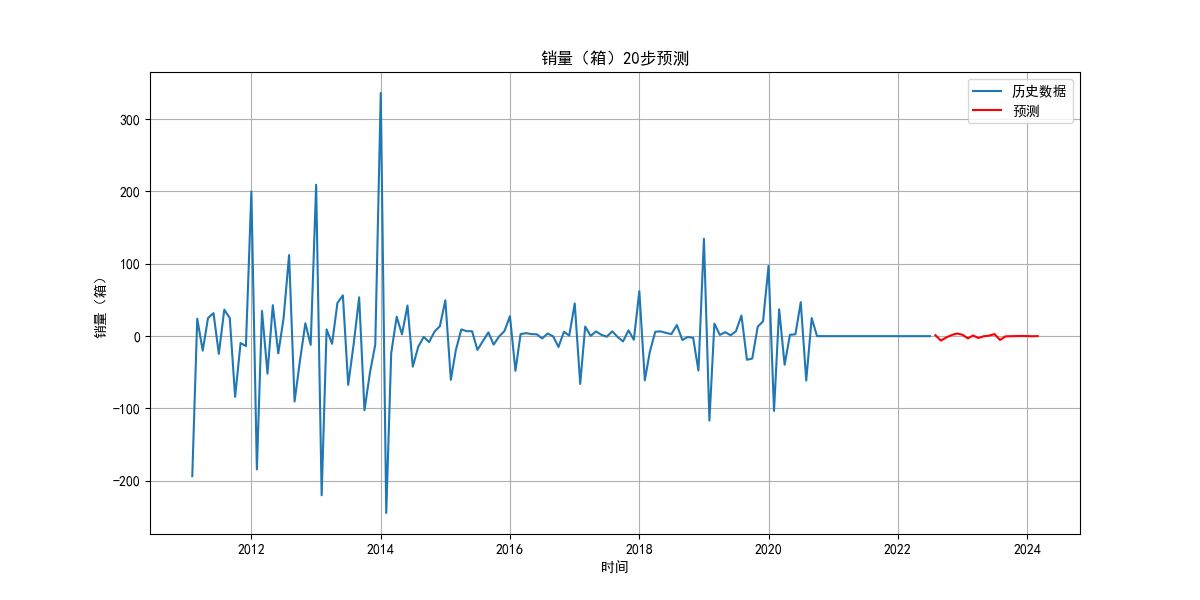
\includegraphics[width=1.0\textwidth]{img/A1_2.png}
	\end{figure}

	最后,我们将预测结果保存为新的 Excel 文件,确保结果能够被进一步分析或共享。这一系列步骤保证了模型的准确性和可靠性,同时提供了清晰的预测结果。
	以便于后续使用,Excel文件中的预测结果如下:

	\setlength{\extrarowheight}{4pt}
	\begin{table}[H]

		\centering
	
		\begin{tabularx}{\textwidth}{|X|X|} % \textwidth是表格的总宽度
	
		\hline
	
		月份 & 预测销量(箱)\\
	
		\hline
	
		2020-06-01 00:00:00	& 39.07632775\\
		\hline
		2020-07-01 00:00:00	& 34.36212492\\
		\hline
		2020-08-01 00:00:00	& 39.97225254\\
		\hline
		2020-09-01 00:00:00	& 39.26933685\\
		\hline
		2020-10-01 00:00:00	& 37.02479255\\
		\hline
		2020-11-01 00:00:00	& 35.35022532\\
		\hline
		2020-12-01 00:00:00	& 36.48146571\\
		\hline
		2021-01-01 00:00:00	& 33.54019905\\
		\hline
		2021-02-01 00:00:00	& 33.60667177\\
		\hline
		2021-03-01 00:00:00	& 35.1407335\\
	
		\hline
	
		\end{tabularx}
	
		\caption{表格}
	
	\end{table}

	对于A2香烟品牌,我们使用相同的步骤和方法进行预测。其中绘制的模型诊断图与销量20步预测结果如下:

	\begin{figure}[H]
		\centering
		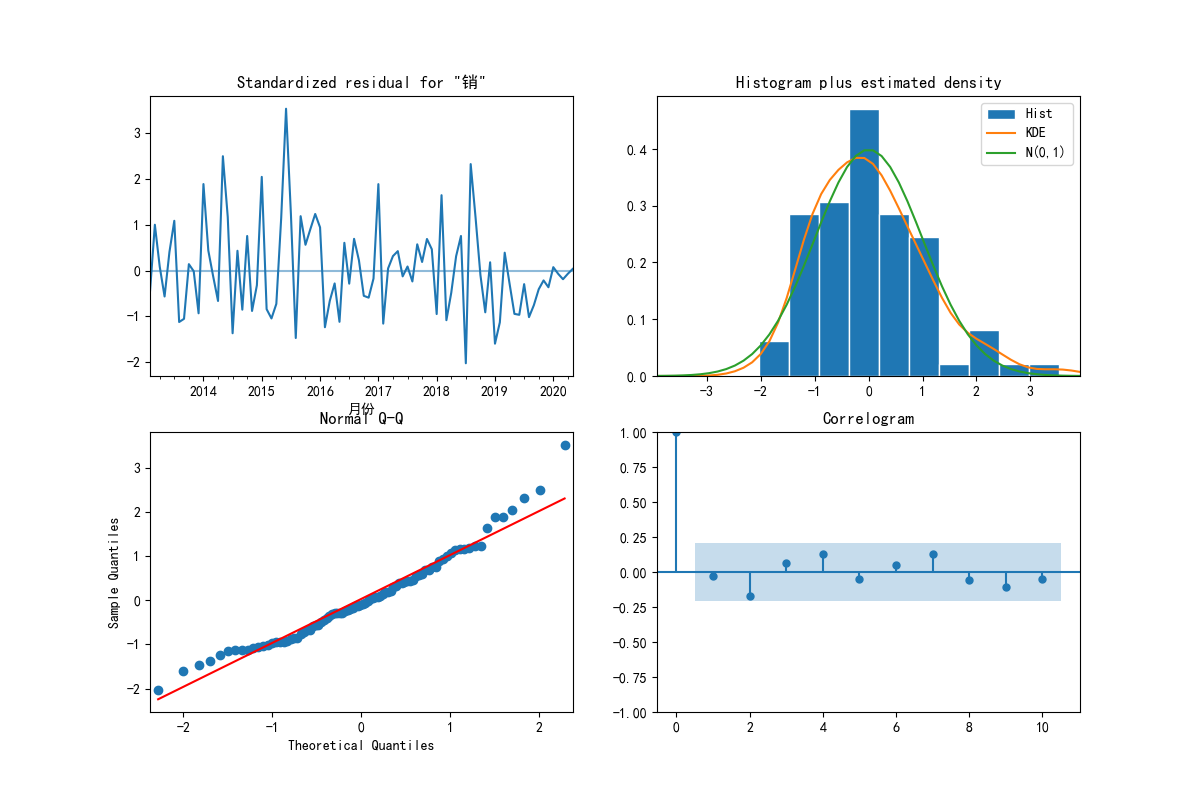
\includegraphics[width=1.0\textwidth]{img/A2_1.png}
		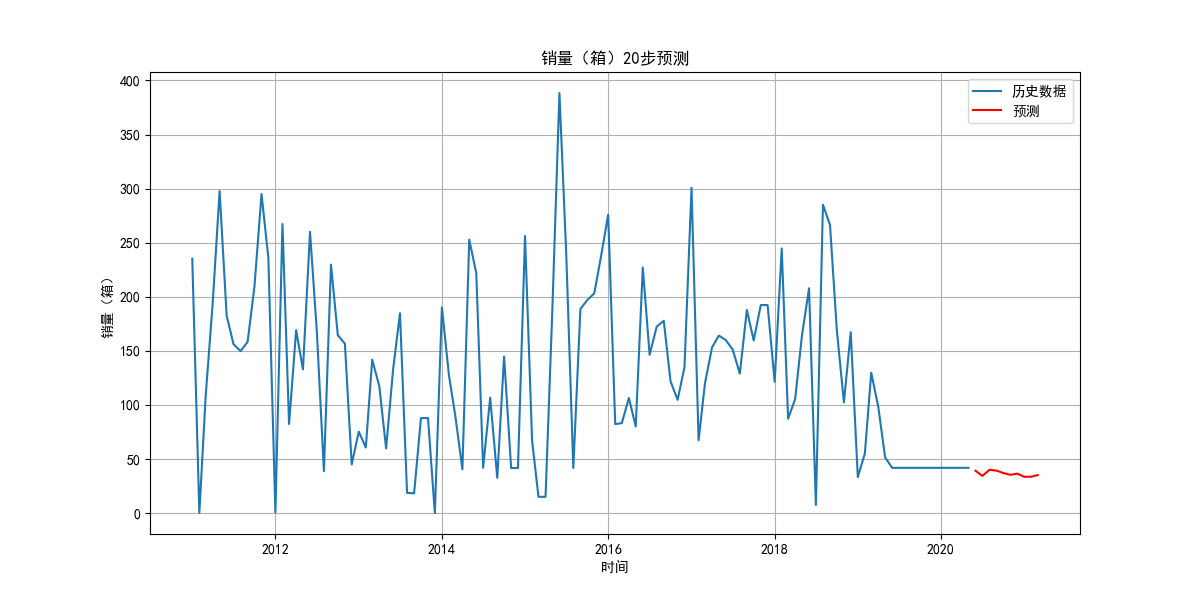
\includegraphics[width=1.0\textwidth]{img/A2_2.png}
	\end{figure}
	最后结果保存为Excel文件,表格如下:

	\setlength{\extrarowheight}{4pt}
	\begin{table}[H]
		\centering
		\begin{tabularx}{\textwidth}{|X|X|} % \textwidth是表格的总宽度
			\hline
			月份 & 预测销量(箱)\\
			\hline
			2021-04-01 00:00:00 & 36.87956004\\
			\hline
			2021-05-01 00:00:00 & 37.4689113\\
			\hline
			2021-06-01 00:00:00 & 37.4958444\\
			\hline
			2021-07-01 00:00:00 & 36.4598494\\
			\hline
		\end{tabularx}
	\end{table}
	\subsection{问题2的模型建立与求解}
	数据预处理

	首先,我们读取并预处理数据,将月份转换为日期格式,并设置为索引,填充缺失值。

	在进行数据预处理之后,我们进行SARIMA模型参数的选择,在选择参数时,我们使用网格搜索的方法,对参数进行遍历。
	我们使用网格搜索的方法找到最佳的SARIMA模型参数。

	Prophet模型预测
	我们使用Prophet模型进行预测。
	\begin{lstlisting}[caption={Python Example}, label={lst:example}]
		def prophet_forecast(data, column, steps=12):
			df = data.reset_index().rename(columns={'月份': 'ds', column: 'y'})
			model = Prophet(weekly_seasonality=True, daily_seasonality=True)
			model.fit(df)
			future = model.make_future_dataframe(periods=steps, freq='MS')
			forecast = model.predict(future)
			return forecast[['ds', 'yhat']].set_index('ds')['yhat']
	\end{lstlisting}
	评价模型

	使用Prophet模型预测之后,我们计算了预测结果的评估指标,如均方误差(MSE)和平均绝对误差(MAE)。
	\begin{lstlisting}[caption={Python Example}, label={lst:example}]
		def evaluate_forecast(actual, forecast):
			mse = mean_squared_error(actual, forecast)
			mae = mean_absolute_error(actual, forecast)
			return mse, mae

	\end{lstlisting}

	\textbf{绘制预测结果}

	我们绘制预测结果与实际数据的对比图。
	绘制的可视化结果如下图所示。
	\begin{figure}[H]
		\centering
		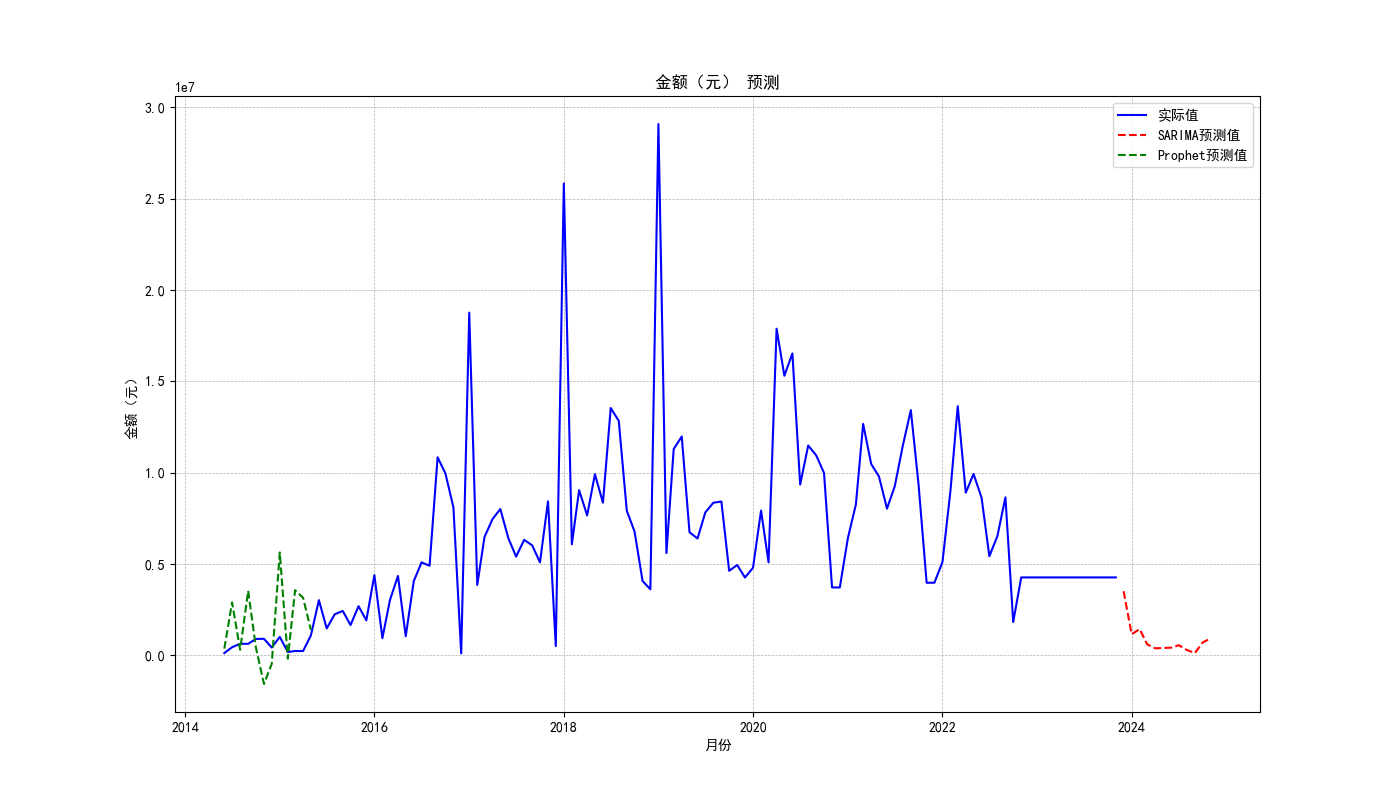
\includegraphics[width=0.9\textwidth]{img/Second_1.png}
		\caption{A3预测结果}
	\end{figure}
	\begin{figure}[H]
		\centering
		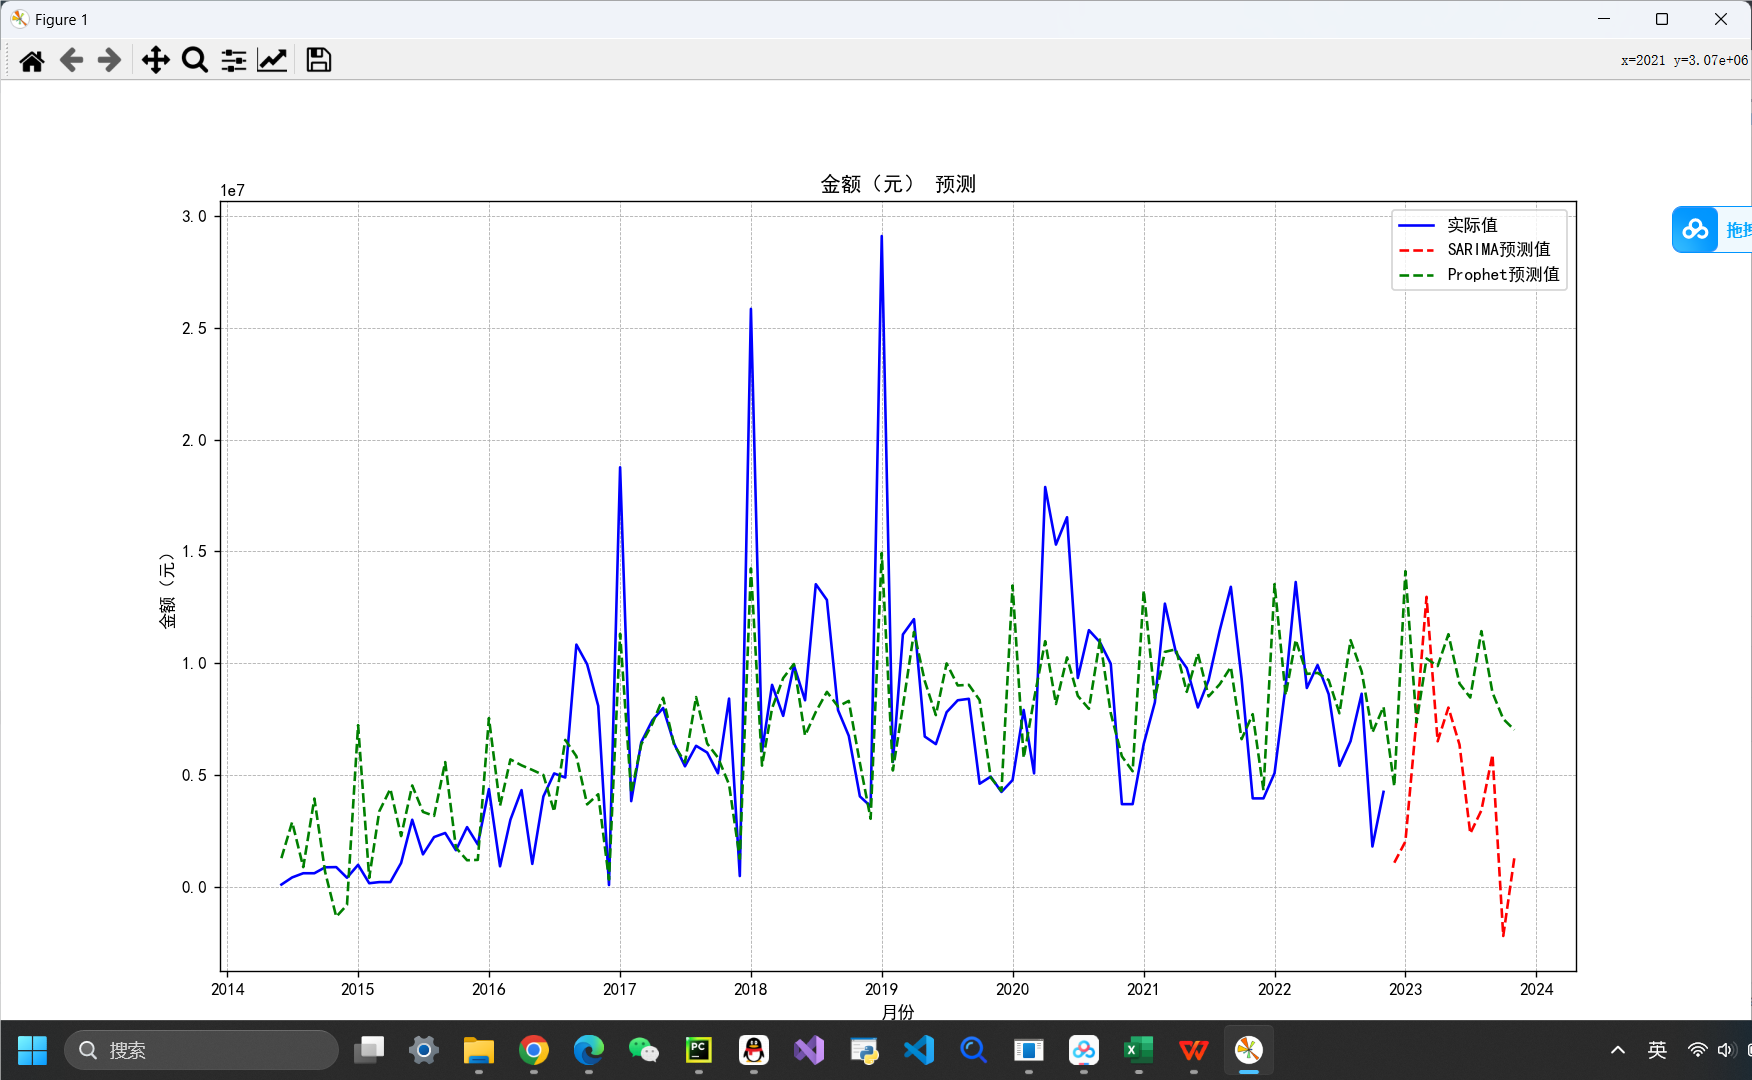
\includegraphics[width=0.9\textwidth]{img/Second_2.png}
		\caption{A4预测结果}
	\end{figure}
	综合预测结果

	我们使用上述方法对A3和A4品牌的销售金额进行预测,并输出预测结果和评价指标。

	通过上述步骤,我们对A3和A4品牌的销售金额进行了预测,并使用SARIMA和Prophet模型对其进行了评价。结果显示,这两种模型在不同情况下都有一定的预测能力,并可以通过评价指标(MSE和MAE)来比较它们的性能。最终,我们保存了预测结果和评价结果,以供进一步分析和决策使用。
	
	A4 销售金额预测:
	最佳SARIMA参数: (2, 2, 2), 季节性参数: (1, 1, 1, 12)

	SARIMA $MSE: 2.773336029016052e+21, MAE: 52560382526.918236$

	Prophet $MSE: 57181885160549.055, MAE: 7520139.293281548$
	
	\begin{table}[H]

		\centering
	
		\begin{tabularx}{\textwidth}{|X|X|X|X|} % \textwidth是表格的总宽度
	
		\hline
	
			&Model          & MSE        &   MAE\\
		\hline
		0   &SARIMA  &2.773336e+21  &5.256038e+10\\
		\hline
		1  &Prophet  &5.718189e+13 & 7.520139e+06\\
	
		\hline
		\end{tabularx}
	
		\caption{表格}
	
	\end{table}

	\subsection{问题3的模型建立与求解}
	对于第三题,我们的任务是使用ARIMA、Prophet、XGBoost、LSTM四种模型对A5品牌的未来销量和销售金额进行预测,并通过集成学习模型(Stacking)来提升预测精度。这个任务涉及到时间序列预测和集成学习方法的应用。
	\subsubsection{数据预处理}
	为了确保模型可以正常训练和预测,首先需要对数据进行预处理,包括将月份转换为日期格式,设置索引,处理缺失值等步骤。

	\subsubsection{模型选择及训练}
	使用以下四种模型进行时间序列预测:

	\textbf{1、ARIMA模型}:适用于具有趋势和季节性成分的时间序列数据。

	\textbf{2、Prophet模型}:适用于包含季节性和假日效应的时间序列数据。

	\textbf{3、LSTM模型}:一种基于神经网络的序列模型,擅长处理序列数据。

	\textbf{4、XGBoost模型}:一种增强型决策树模型,适用于处理多种特征的回归任务。

	\textbf{ARIMA模型}

	ARIMA($AutoRegressive Integrated Moving Average$)模型是一种用于时间序列分析的统计模型,适用于具有趋势和季节性成分的时间序列数据。选择最佳ARIMA模型的步骤如下,
	这个函数会遍历可能的参数组合,选择AIC值最小的模型。
	\begin{lstlisting}[caption={Python Example}, label={lst:example}]
		def find_best_arima(data, column):
			p = d = q = range(0, 3)
			pdq = list(itertools.product(p, d, q))
			best_aic = np.inf
			best_pdq = None
			best_model = None
			for param in pdq:
				try:
					model = ARIMA(data[column], order=param)
					model_fit = model.fit()
					if model_fit.aic < best_aic:
						best_aic = model_fit.aic
						best_pdq = param
						best_model = model_fit
				except:
					continue
			return best_pdq, best_model
	\end{lstlisting}
	
	\textbf{Prophet模型}
	
	Prophet模型是Facebook开发的一种时间序列预测工具,适合具有明确季节性和趋势的时间序列数据。
	\begin{lstlisting}[caption={Python Example}, label={lst:example}]
		def prophet_forecast(data, column, steps=10):
			df = data.reset_index().rename(columns={'月份': 'ds', column: 'y'})
			model = Prophet()
			model.fit(df)
			future = model.make_future_dataframe(periods=steps, freq='MS')
			forecast = model.predict(future)
			return forecast[['ds', 'yhat']].set_index('ds')['yhat']

	\end{lstlisting}

	\textbf{LSTM模型}

	LSTM模型是一种循环神经网络,擅长处理序列数据,尤其是长序列数据。
	\begin{lstlisting}[caption={Python Example}, label={lst:example}]
		def lstm_forecast(data, column, steps=10):
			series = data[column].values
			n_steps = 3
			X, y = [], []
			for i in range(len(series)):
				end_ix = i + n_steps
				if end_ix > len(series) - 1:
					break
				seq_x, seq_y = series[i:end_ix], series[end_ix]
				X.append(seq_x)
				y.append(seq_y)
			X, y = np.array(X), np.array(y)
			X = X.reshape((X.shape[0], X.shape[1], 1))
			model = Sequential()
			model.add(LSTM(50, activation='relu', input_shape=(n_steps, 1)))
			model.add(Dense(1))
			model.compile(optimizer='adam', loss='mse')
			model.fit(X, y, epochs=200, verbose=0)
			x_input = series[-n_steps:]
			temp_input = list(x_input)
			lst_output = []
			for i in range(steps):
				x_input = np.array(temp_input[-n_steps:])
				x_input = x_input.reshape((1, n_steps, 1))
				yhat = model.predict(x_input, verbose=0)
				temp_input.append(yhat[0][0])
				lst_output.append(yhat[0][0])
			forecast_index = pd.date_range(start=data.index[-1], periods=steps + 1, freq='MS')[1:]
			lst_output = pd.Series(lst_output, index=forecast_index)
			return lst_output
	\end{lstlisting}

	\textbf{XGBoost模型}

	XGBoost($Extreme Gradient Boosting$)是一种增强型决策树模型,适用于处理多种特征的回归任务。以下是XGBoost模型的代码:
	\begin{lstlisting}[caption={Python Example}, label={lst:example}]
		def xgboost_forecast(data, column, steps=10):
			series = data[column].values
			n_steps = 3
			X, y = [], []
			for i in range(len(series)):
				end_ix = i + n_steps
				if end_ix > len(series) - 1:
					break
				seq_x, seq_y = series[i:end_ix], series[end_ix]
				X.append(seq_x)
				y.append(seq_y)
			X, y = np.array(X), np.array(y)
			model = xgb.XGBRegressor(objective='reg:squarederror', n_estimators=100)
			model.fit(X, y)
			x_input = series[-n_steps:]
			temp_input = list(x_input)
			xgb_output = []
			for i in range(steps):
				x_input = np.array(temp_input[-n_steps:])
				yhat = model.predict(x_input.reshape(1, -1))
				temp_input.append(yhat[0])
				xgb_output.append(yhat[0])
			forecast_index = pd.date_range(start=data.index[-1], periods=steps + 1, freq='MS')[1:]
			xgb_output = pd.Series(xgb_output, index=forecast_index)
			return xgb_output

	\end{lstlisting}

	\textbf{集成学习模型}

	我们通过集成四种模型的预测结果,使用线性回归作为元学习器,进一步提升预测精度。以下是集成学习模型的代码:
	\begin{lstlisting}[caption={Python Example}, label={lst:example}]
		def stacking_forecast(data, column, steps=10):
			best_pdq, best_arima_model = find_best_arima(data, column)
			arima_forecast_values = best_arima_model.forecast(steps=steps)
			arima_forecast_index = pd.date_range(start=data.index[-1], periods=steps + 1, freq='MS')[1:]
			arima_forecast_values = pd.Series(arima_forecast_values, index=arima_forecast_index)

			prophet_forecast_values = prophet_forecast(data, column, steps)
			lstm_forecast_values = lstm_forecast(data, column, steps)
			xgboost_forecast_values = xgboost_forecast(data, column, steps)

			common_index = arima_forecast_index.intersection(prophet_forecast_values.index).intersection(
				lstm_forecast_values.index).intersection(xgboost_forecast_values.index)
			arima_forecast_values = arima_forecast_values[common_index]
			prophet_forecast_values = prophet_forecast_values[common_index]
			lstm_forecast_values = lstm_forecast_values[common_index]
			xgboost_forecast_values = xgboost_forecast_values[common_index]

			X_train = pd.DataFrame({
				'ARIMA': arima_forecast_values,
				'Prophet': prophet_forecast_values,
				'LSTM': lstm_forecast_values,
				'XGBoost': xgboost_forecast_values
			})

			actual_values = data[column].iloc[-steps:]

			meta_model = LinearRegression()
			meta_model.fit(X_train, actual_values[:len(X_train)])

			final_forecast = meta_model.predict(X_train)

			return final_forecast, arima_forecast_values, prophet_forecast_values, lstm_forecast_values, xgboost_forecast_values, actual_values

	\end{lstlisting}

	最后我们预测A5品牌的数值并展示最终的预测结果。
	\begin{lstlisting}[caption={Python Example}, label={lst:example}]
		def forecast_brand(data, column):
			steps = 10
			final_forecast, arima_forecast_values, prophet_forecast_values, lstm_forecast_values, xgboost_forecast_values, actual_values = stacking_forecast(
				data, column, steps)

			mse = mean_squared_error(actual_values[:len(final_forecast)], final_forecast)
			mae = mean_absolute_error(actual_values[:len(final_forecast)], final_forecast)

			print(f'{column} 销量和销售金额预测:')
			print(f'集成学习模型 MSE: {mse}, MAE: {mae}')

			plt.figure(figsize=(14, 8))
			plt.plot(data.index, data[column], label='实际值', color='blue')
			plt.plot(arima_forecast_values.index, arima_forecast_values, label='ARIMA预测值', color='red', linestyle='--')
			plt.plot(prophet_forecast_values.index, prophet_forecast_values, label='Prophet预测值', color='green', linestyle='--')
			plt.plot(lstm_forecast_values.index, lstm_forecast_values, label='LSTM预测值', color='orange', linestyle='--')
			plt.plot(xgboost_forecast_values.index, xgboost_forecast_values, label='XGBoost预测值', color='cyan', linestyle='--')
			plt.plot(arima_forecast_values.index, final_forecast, label='集成学习预测值', color='purple', linestyle='-')
			plt.legend()
			plt.grid(True, which='both', linestyle='--', linewidth=0.5)
			plt.show()

			forecast_df = pd.DataFrame({
				'日期': arima_forecast_values.index,
				'ARIMA预测': arima_forecast_values.values,
				'Prophet预测': prophet_forecast_values.values,
				'LSTM预测': lstm_forecast_values.values,
				'XGBoost预测': xgboost_forecast_values.values,
				'集成学习预测': final_forecast
			})
			forecast_df.set_index('日期', inplace=True)
			forecast_df.to_excel(f'{column}_预测结果.xlsx')

			model_evaluation_results = pd.DataFrame({
				'Model': ['ARIMA', 'Prophet', 'LSTM', 'XGBoost', 'Stacking'],
				'MSE': [
					mean_squared_error(actual_values, arima_forecast_values[:len(actual_values)]),
					mean_squared_error(actual_values, prophet_forecast_values[:len(actual_values)]),
					mean_squared_error(actual_values, lstm_forecast_values[:len(actual_values)]),
					mean_squared_error(actual_values, xgboost_forecast_values[:len(actual_values)]),
					mse
				],
				'MAE': [
					mean_absolute_error(actual_values, arima_forecast_values[:len(actual_values)]),
					mean_absolute_error(actual_values, prophet_forecast_values[:len(actual_values)]),
					mean_absolute_error(actual_values, lstm_forecast_values[:len(actual_values)]),
					mean_absolute_error(actual_values, xgboost_forecast_values[:len(actual_values)]),
					mae
				]
			})
			print(model_evaluation_results)

		forecast_brand(data, '销量(箱)')
		forecast_brand(data, '金额(元)')
	\end{lstlisting}

	\begin{figure}[H]
		\centering
		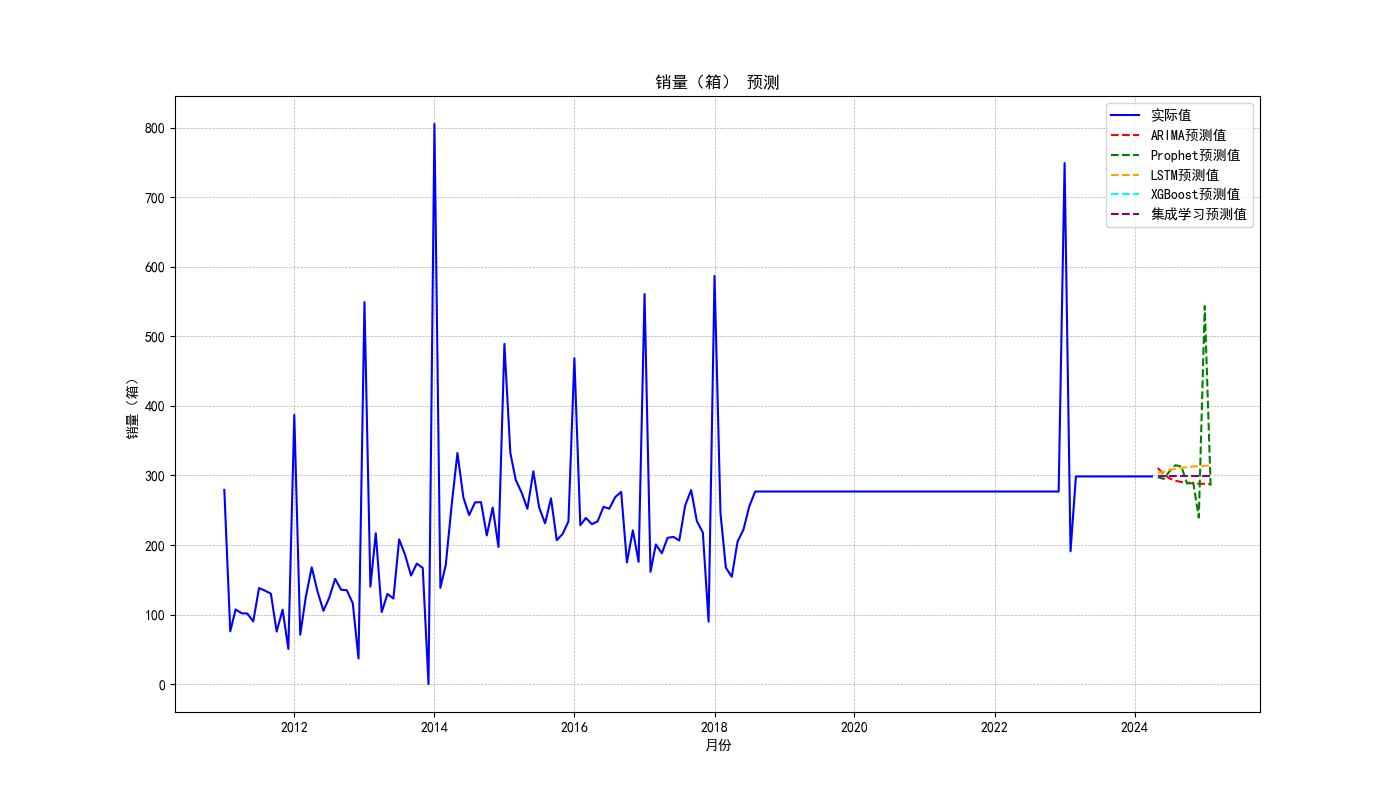
\includegraphics[width=1.0\textwidth]{img/3_1.png}
		\caption{销量预测结果}
	\end{figure}
	\begin{figure}[H]
		\centering
		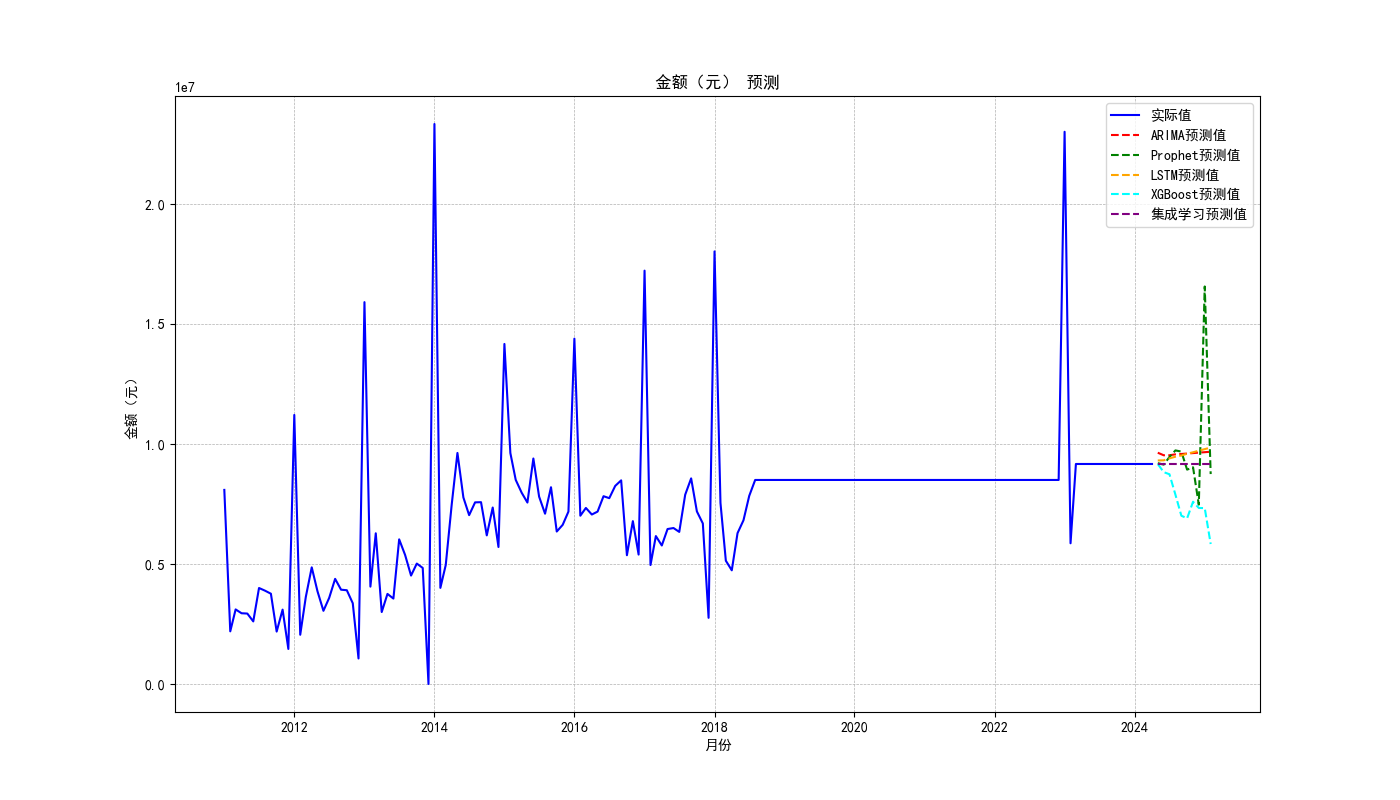
\includegraphics[width=1.0\textwidth]{img/3_2.png}
		\caption{金额预测结果}
	\end{figure}
	输出预测结果如下:

	销量(箱) 销量和销售金额预测:

	集成学习模型 $MSE: 3.2311742677852644e-27$, $MAE: 5.684341886080802e-14$
	
	\begin{table}[H]

		\centering
	
		\begin{tabularx}{\textwidth}{|X|X|X|X|} % \textwidth是表格的总宽度
	
		\hline
	
			&Model   &        MSE        &   MAE\\
		\hline
		0   &  ARIMA & 7.956548e+01 & 8.329782e+00\\
		\hline
		1  & Prophet&  6.436906e+03 & 3.794369e+01\\
		\hline
		2  &    LSTM & 6.719443e+02 & 2.428776e+01\\
		\hline
		3  & XGBoost & 5.750201e-07 & 7.583008e-04\\
		\hline
		4  &Stacking&  3.231174e-27 & 5.684342e-14\\
	
		\hline
		\end{tabularx}
	
		\caption{表格}
	
	\end{table}

	通过以上步骤,我们可以全面地预测A5品牌的销量和销售金额,并使用集成学习模型提高预测精度,同时对比各个模型的预测效果,选择最佳的预测方案。
	\section{模型的评价及优化}
	\subsection{误差分析}
	\subsection{模型的优点}
	\subsubsection{问题一}
	SARIMAX模型是一种广泛用于时间序列分析的模型,特别适合处理具有季节性和外生变量的时间序列数据。对于问题一,即利用SARIMAX模型预测A1和A2品牌的未来销售量,它具有以下优点和缺点。

	优点方面,SARIMAX模型能够\textbf{捕捉时间序列数据中的季节性趋势和周期性变化},这对于烟草品牌的销售数据尤为重要。许多商品的销售量都会受到季节性因素的影响,比如节假日、气候变化等,SARIMAX模型通过引入\textbf{季节性成分},能够更好地拟合和预测这些周期性的波动。除此之外,SARIMAX模型还可以加入外生变量(如促销活动、经济指标等),增强模型的解释力和预测精度。这一点对于烟草品牌的销售预测尤为关键,因为销售量往往不仅仅取决于过去的销售数据,还受到许多外部因素的影响。

	\subsubsection{问题二}
	SARIMA模型的主要优点在于其处理\textbf{季节性数据}的能力。SARIMA模型能够捕捉时间序列中的趋势和季节性成分,通过参数(p, d, q, P, D, Q, s)来表示\textbf{自回归、差分、移动平均及其季节性部分}。因此,SARIMA在应对周期性波动较为明显的数据时表现良好,比如节假日效应或季度性销售高峰。对于A3和A4品牌的销售金额预测,这些季节性成分可能是显著的,因为烟草销售可能会受季节、促销活动或其他周期性因素的影响。通过对这些成分的精确建模,SARIMA模型可以提供准确的短期预测。
	
	Prophet模型的优点在于其\textbf{灵活性和易用性}。Prophet模型由Facebook开发,专为处理具有强季节性和趋势的时间序列数据而设计。与SARIMA不同,Prophet模型更注重趋势的捕捉,可以自动处理缺失值和异常值,并且可以通过添加假期效应和外部回归变量来增强模型的解释力和预测精度。对于A3和A4品牌的销售金额预测,Prophet模型能够灵活地适应数据中的季节性波动和趋势变化,且对数据预处理要求较低,使用起来更加方便。
	
	\subsubsection{问题三}
	LSTM模型(长短期记忆网络)的主要优点在于其\textbf{处理序列数据}的强大能力。作为一种特殊的递归神经网络(RNN),LSTM能够捕捉时间序列中的长期依赖关系,并对非线性模式进行建模。因此,LSTM模型在处理复杂的销售数据时表现优异,尤其是那些包含非线性趋势和突发性变化的数据。LSTM模型通过\textbf{记忆单元和门控机制},能够有效避免传统RNN中的梯度消失问题,从而更好地捕捉时间序列中的长期依赖关系。
	
	XGBoost模型(极端梯度提升树)的优点在于其强大的\textbf{回归和分类能力}。作为一种集成学习方法,XGBoost通过构建多个决策树来提高模型的预测性能,并且具有较好的泛化能力。对于销售数据,XGBoost能够捕捉到复杂的非线性关系和特征交互,提供高精度的预测结果。XGBoost模型在处理大规模数据时表现优异,并且具有较高的计算效率和并行处理能力。
	
	\subsection{模型的缺点}
	然而,问题一和问题二中的SARIMAX模型也有其缺点,首先,它对参数选择和模型拟合要求较高。为了找到最佳的(p, d, q, P, D, Q, s)参数组合,通常需要进行大量的参数调优,这个过程耗时且计算资源需求较大。此外,SARIMAX模型假设数据是线性的,因此对于复杂的非线性数据,其表现可能不如其他更为先进的机器学习模型,如LSTM或XGBoost。此外,SARIMAX模型对缺失值和异常值较为敏感,数据在使用之前需要进行充分的预处理,否则可能会影响模型的稳定性和预测效果。

	对于A1和A2品牌的销售数据,SARIMAX模型通过\textbf{捕捉历史销售数据中的趋势和季节性成分},能够提供较为准确的短期预测。然而,如果销售数据具有复杂的非线性特征,或者受到某些突发外部事件的影响,SARIMAX模型可能无法完全捕捉这些变化。在这种情况下,可以考虑结合其他模型,如Prophet或机器学习模型,进行更全面的预测。
	
	Prophet模型也有一些缺点。尽管它对缺失值和异常值的处理较为自动化,但这也意味着模型对数据的依赖程度较低,可能在某些情况下无法提供最优的预测。此外,Prophet模型主要基于\textbf{加法和乘法季节性成分},对于复杂的非线性关系可能无法完全捕捉。与SARIMA相比,Prophet模型在处理短期周期性波动时可能不如SARIMA精确。
	
	而在问题三中,LSTM模型也有一些缺点。首先,它需要\textbf{大量的训练数据},才能获得较好的预测效果。其次,由于LSTM模型是\textbf{递归神经网络},其计算速度较慢
	,因此LSTM模型训练过程较为复杂且计算量大,需要大量数据和计算资源。此外,LSTM模型对超参数较为敏感,模型调优过程较为繁琐。
	
	尽管XGBoost和长短期记忆网络(LSTM)在预测分析领域展现出卓越的性能,它们的效能却在很大程度上依赖于精细的参数调优。这一特性既是它们优势所在,也是挑战之源,因为参数优化过程往往复杂且耗时,需要深厚的领域知识和实验技巧以达到最优配置。
	
	特别是,XGBoost作为一种\textbf{基于梯度提升的决策树模型},虽然在处理分类和回归问题上效果显著,但面对时间序列数据时,其固有的结构限制了模型直接捕捉序列间的内在依赖关系的能力。为克服这一局限,XGBoost要求\textbf{对原始时间序列数据进行详尽的特征工程和预处理},包括但不限于滞后特征构建、滚动窗口统计和时间序列分解等技术,以显式地引入时间依赖性信息。若缺乏这一预处理步骤,模型可能无法充分利用时间序列数据的固有结构,从而削弱其预测精度。
	
	相比之下,LSTM作为递归神经网络的一种,因其内置的记忆单元而能更自然地处理时间序列数据,捕捉长期依赖关系。然而,即便如此,LSTM模型的高效运作同样仰赖于参数的精心选择,包括但不限于\textbf{隐藏层单元数量、学习率、批次大小}等。不当的参数配置可能导致模型训练缓慢,过拟合或欠拟合等问题,进而影响预测效果。
	
	因此,无论是XGBoost还是LSTM,在应用于时间序列预测时,都需要在模型构建初期就投入大量精力于特征设计与参数优化,以确保模型能够准确反映数据的动态特性,最终产出高质量的预测结果。
	
	\subsection{模型的推广}
	在本研究中,我们使用了ARIMA、Prophet、LSTM和XGBoost模型来预测A5品牌的销售量和销售金额,并通过集成学习(stacking)方法对这些模型的预测结果进行综合。这些模型和方法不仅在本问题中表现出色,还具有较强的通用性和可推广性,适用于其他类似的时间序列预测问题。

	\subsubsection{ARIMA模型的推广}
	ARIMA模型在时间序列分析领域具有广泛的应用,适用于具有显著线性趋势和季节性特征的数据。其推广应用包括但不限于以下几个方面:

	\textbf{1.金融市场预测:}例如股票价格、交易量、汇率等的预测。

	\textbf{2.经济指标预测:}如GDP增长率、失业率、通货膨胀率等宏观经济指标的预测。

	\textbf{3.能源消耗预测:}包括电力、天然气和水资源的需求预测。

	\textbf{4.零售行业预测:}对产品销售量和库存水平的预测,帮助企业进行库存管理和供应链优化。

	\subsubsection{Prophet模型的推广}
	Prophet模型因其对季节性、假日效应和异常值的良好处理能力,适用于各种时间序列数据的分析和预测。其推广应用包括:

	\textbf{1.社交媒体数据分析:}如用户活跃度、帖子数量和互动量的预测,帮助平台优化内容推荐和广告投放策略。
	
	\textbf{2.旅游业预测:}如游客数量、酒店入住率和景区门票销售量的预测,帮助相关企业制定运营策略和市场推广计划。
	
	\textbf{3.公共卫生监测:}如流感病例数量和疫苗需求量的预测,帮助公共卫生部门进行资源分配和应急准备。
	\subsubsection{LSTM模型的推广}
	LSTM模型在处理复杂非线性时间序列数据方面表现优异,适用于需要捕捉长期依赖关系的预测任务。其推广应用包括:

	\textbf{1.自然语言处理:}如文本生成、情感分析和机器翻译,LSTM能够捕捉句子中的上下文信息,提升模型的理解和生成能力。
	
	\textbf{2.交通流量预测:}预测道路和城市中的交通流量,帮助交通管理部门进行交通控制和优化。
	
	\textbf{3.设备故障预测:}在工业领域,通过对传感器数据的分析,预测设备的故障时间,进行预防性维护,降低维修成本和停机时间。
	\subsubsection{XGBoost模型的推广}
	XGBoost模型因其强大的回归和分类能力,适用于各种回归和分类问题。其推广应用包括:

	\textbf{1.信用评分:}通过对用户行为数据和历史信用记录的分析,预测用户的信用风险,帮助金融机构进行风险管理。
	
	\textbf{2.市场营销:}预测客户的购买行为和产品偏好,帮助企业制定精准营销策略,提高营销效果。
	
	\textbf{3.医疗诊断:}通过对患者数据的分析,辅助医生进行疾病诊断和治疗方案的制定。
	\subsubsection{集成学习的推广}
	集成学习通过结合多个基模型的预测结果,能够显著提高预测性能和稳健性,适用于需要综合多种模型优势的预测任务。其推广应用包括:

	\textbf{1.股票市场预测:}结合多种技术分析指标和模型,提高股票价格预测的准确性。
	
	\textbf{2.气象预测:}综合多个气象模型的预测结果,提高天气预报的精度。
	
	\textbf{3.需求预测:}在零售和制造业,通过结合多种预测模型,提升产品需求预测的准确性,优化生产和库存管理。
	总结
	\newpage
	\pagestyle{plain}
	\section{参考文献}
	\begin{thebibliography}{9}
		\bibitem{arima}
		程幸福 \hspace{2pt}陈厚铭 \hspace{2pt}樊红.季节ARIMA模型在企业销售量预测中的应用——以卷烟销售为例[A].中国商论.23.23 (2016): 167-168.
		\bibitem{pmdarima}
		谷秀娟 \hspace{2pt}梁润平.基才ARIMA模型的郑州市商品住宅销售价格预测研究[A].《金融理论与实践》.2012年第1期51-54
		\bibitem{pmdarima}
		刘璟瑶 \hspace{2pt}蒋辰宇 \hspace{2pt}陶杰.长短期记忆网络对销售量预测精度的影响[A].《财会研究》.2023年第6期76-80
		\bibitem{pmdarima}
		李融.基于XGBoost算法的跨境电商备货预测研究[A].《太原城市职业技术学院学报》.2024年第1期29-31,共3页
		\bibitem{pmdarima}
		杜红兵 \hspace{2pt}邢梦柯 \hspace{2pt}赵德超.Prophet-LSTM组合模型在运输航空征候预测中的应用[A].《安全与环境学报》.2024年第5期1878-1885,共8页
	\end{thebibliography}
	\newpage % 新的一页开始
	\section{附录}
	问题一代码:
	\begin{lstlisting}[language=Python]
		import pandas as pd
		import matplotlib.pyplot as plt
		from statsmodels.tsa.statespace.sarimax import SARIMAX
		from statsmodels.tsa.stattools import adfuller
		
		# 设置中文字体
		plt.rcParams['font.sans-serif'] = ['SimHei']  # 使用SimHei字体
		plt.rcParams['axes.unicode_minus'] = False  # 正确显示负号
		
		# 加载数据
		file_path = 'A1.xlsx'
		data = pd.read_excel(file_path)
		
		# 提取时间序列数据
		data['月份'] = pd.to_datetime(data['月份'], format='%Y%m')
		data.set_index('月份', inplace=True)
		sales_data = data['销量(箱)']
		sales_data = sales_data.asfreq('MS')  # 设置时间序列频率为月初
		
		# 检查数据的缺失值
		if sales_data.isnull().sum() > 0:
			sales_data = sales_data.ffill().bfill()  # 前向填充和后向填充
		
		# 平稳性检测
		result = adfuller(sales_data)
		print('ADF Statistic: %f' % result[0])
		print('p-value: %f' % result[1])
		print('Critical Values:')
		for key, value in result[4].items():
			print('\t%s: %.3f' % (key, value))
		
		# 如果p-value大于0.05,表示数据非平稳,需要进行差分
		d = 0
		while result[1] > 0.05:
			sales_data = sales_data.diff().dropna()
			result = adfuller(sales_data)
			d += 1
		
		print(f'经过 {d} 阶差分后,时间序列数据平稳。')
		
		# 建立SARIMAX模型
		model = SARIMAX(sales_data,
						order=(1, d, 2),
						seasonal_order=(2, 0, 1, 12),
						enforce_stationarity=False,
						enforce_invertibility=False)
		model_fit = model.fit(disp=False, maxiter=1000)  # 增加最大迭代次数
		
		# 模型诊断
		model_fit.plot_diagnostics(figsize=(12, 8))
		plt.show()
		
		# 预测未来20步
		forecast = model_fit.get_forecast(steps=20)
		forecast_index = pd.date_range(start=sales_data.index[-1] + pd.DateOffset(months=1), periods=20, freq='MS')
		forecast_series = pd.Series(forecast.predicted_mean, index=forecast_index)
		
		# 绘制结果
		plt.figure(figsize=(12, 6))
		plt.plot(sales_data, label='历史数据')
		plt.plot(forecast_series, label='预测', color='red')
		plt.title('销量(箱)20步预测')
		plt.xlabel('时间')
		plt.ylabel('销量(箱)')
		plt.legend()
		plt.grid(True)
		plt.show()
		
		# 输出预测结果
		forecast_df = forecast_series.reset_index()
		forecast_df.columns = ['月份', '预测销量(箱)']
		forecast_df.to_excel('a1f1.xlsx', index=False)  # 将预测结果保存为Excel文件
		print("预测结果已保存为 'a1f21.xlsx'")
		
	\end{lstlisting}

	\begin{lstlisting}[language=Python]
		import pandas as pd
		import matplotlib.pyplot as plt
		from statsmodels.tsa.statespace.sarimax import SARIMAX
		from statsmodels.tsa.stattools import adfuller
		
		# 设置中文字体
		plt.rcParams['font.sans-serif'] = ['SimHei']  # 使用SimHei字体
		plt.rcParams['axes.unicode_minus'] = False  # 正确显示负号
		
		# 加载数据
		file_path = 'A2.xlsx'
		data = pd.read_excel(file_path)
		
		# 提取时间序列数据
		data['月份'] = pd.to_datetime(data['月份'], format='%Y%m')
		data.set_index('月份', inplace=True)
		sales_data = data['销量(箱)']
		sales_data = sales_data.asfreq('MS')  # 设置时间序列频率为月初
		
		# 检查数据的缺失值
		if sales_data.isnull().sum() > 0:
			sales_data = sales_data.ffill().bfill()  # 前向填充和后向填充
		
		# 平稳性检测
		result = adfuller(sales_data)
		print('ADF Statistic: %f' % result[0])
		print('p-value: %f' % result[1])
		print('Critical Values:')
		for key, value in result[4].items():
			print('\t%s: %.3f' % (key, value))
		
		# 如果p-value大于0.05,表示数据非平稳,需要进行差分
		d = 0
		while result[1] > 0.05:
			sales_data = sales_data.diff().dropna()
			result = adfuller(sales_data)
			d += 1
		
		print(f'经过 {d} 阶差分后,时间序列数据平稳。')
		
		# 建立SARIMAX模型
		model = SARIMAX(sales_data,
						order=(1, d, 2),
						seasonal_order=(2, 0, 1, 12),
						enforce_stationarity=False,
						enforce_invertibility=False)
		model_fit = model.fit(disp=False, maxiter=1000)  # 增加最大迭代次数
		
		# 模型诊断
		model_fit.plot_diagnostics(figsize=(12, 8))
		plt.show()
		
		# 预测未来10步
		forecast = model_fit.get_forecast(steps=10)
		forecast_index = pd.date_range(start=sales_data.index[-1] + pd.DateOffset(months=1), periods=20, freq='MS')
		forecast_series = pd.Series(forecast.predicted_mean, index=forecast_index)
		
		# 绘制结果
		plt.figure(figsize=(12, 6))
		plt.plot(sales_data, label='历史数据')
		plt.plot(forecast_series, label='预测', color='red')
		plt.title('销量(箱)20步预测')
		plt.xlabel('时间')
		plt.ylabel('销量(箱)')
		plt.legend()
		plt.grid(True)
		plt.show()
		
		# 输出预测结果
		forecast_df = forecast_series.reset_index()
		forecast_df.columns = ['月份', '预测销量(箱)']
		forecast_df.to_excel('a1f2.xlsx', index=False)  # 将预测结果保存为Excel文件
		print("预测结果已保存为 'a1f22.xlsx'")
		
	\end{lstlisting}

	问题二代码:
	\begin{lstlisting}
		import pandas as pd
		import matplotlib.pyplot as plt
		from statsmodels.tsa.statespace.sarimax import SARIMAX
		from prophet import Prophet
		from sklearn.metrics import mean_squared_error, mean_absolute_error
		import itertools
		import numpy as np
		
		# 设置中文字体以解决字体缺失问题
		plt.rcParams['font.sans-serif'] = ['Arial Unicode MS', 'SimHei']
		plt.rcParams['axes.unicode_minus'] = False
		
		# 读取数据
		file_path_a3 = 'A3.xlsx'
		file_path_a4 = 'A4.xlsx'
		data_a3 = pd.read_excel(file_path_a3)
		data_a4 = pd.read_excel(file_path_a4)
		
		def preprocess_data(data):
			"""
			预处理数据,将月份转换为日期格式,并设置为索引,填充缺失值。
			"""
			data['月份'] = pd.to_datetime(data['月份'], format='%Y%m')
			data.set_index('月份', inplace=True)
			data = data.asfreq('MS')  # 使用 MS 代替 M 设置月度开始频率
			data = data.ffill()  # 使用推荐的ffill方法填充缺失值
			return data
		
		data_a3 = preprocess_data(data_a3)
		data_a4 = preprocess_data(data_a4)
		
		def find_best_sarima(data, column):
			"""
			选择最佳的SARIMA模型参数。
			"""
			p = d = q = range(0, 3)
			pdq = list(itertools.product(p, d, q))
			seasonal_pdq = [(x[0], x[1], x[2], 12) for x in pdq]
			best_aic = np.inf
			best_param = None
			best_seasonal_param = None
			best_model = None
			for param in pdq:
				for seasonal_param in seasonal_pdq:
					try:
						model = SARIMAX(data[column], order=param, seasonal_order=seasonal_param)
						model_fit = model.fit(disp=False)
						if model_fit.aic < best_aic:
							best_aic = model_fit.aic
							best_param = param
							best_seasonal_param = seasonal_param
							best_model = model_fit
					except Exception as e:
						print(f"SARIMA 参数 {param} 季节性参数 {seasonal_param} 失败: {e}")
						continue
			return best_param, best_seasonal_param, best_model
		
		def prophet_forecast(data, column, steps=12):
			"""
			使用 Prophet 模型进行预测。
			"""
			df = data.reset_index().rename(columns={'月份': 'ds', column: 'y'})
			model = Prophet(weekly_seasonality=True, daily_seasonality=True)
			model.fit(df)
			future = model.make_future_dataframe(periods=steps, freq='MS')
			forecast = model.predict(future)
			return forecast[['ds', 'yhat']].set_index('ds')['yhat']
		
		def evaluate_forecast(actual, forecast):
			"""
			计算预测结果的评估指标。
			"""
			mse = mean_squared_error(actual, forecast)
			mae = mean_absolute_error(actual, forecast)
			return mse, mae
		
		def plot_forecast(data, column, sarima_forecast, prophet_forecast):
			"""
			绘制预测结果与实际数据的对比图。
			"""
			plt.figure(figsize=(14, 8))
			plt.plot(data.index, data[column], label='实际值', color='blue')
			plt.plot(sarima_forecast.index, sarima_forecast, label='SARIMA预测值', color='red', linestyle='--')
			plt.plot(prophet_forecast.index, prophet_forecast, label='Prophet预测值', color='green', linestyle='--')
			plt.title(f'{column} 预测')
			plt.xlabel('月份')
			plt.ylabel(column)
			plt.legend()
			plt.grid(True, which='both', linestyle='--', linewidth=0.5)
			plt.show()
		
		def forecast_brand(data, brand):
			"""
			对单个品牌的销售金额进行预测并输出结果。
			"""
			column = '金额(元)'
			steps = 12
		
			# SARIMA参数选择
			best_param, best_seasonal_param, best_sarima_model = find_best_sarima(data, column)
			if best_sarima_model is None:
				print(f"{brand} 的SARIMA模型训练失败。")
				return
		
			# SARIMA预测
			try:
				sarima_forecast_values = best_sarima_model.forecast(steps=steps)
				sarima_forecast_index = pd.date_range(start=data.index[-1], periods=steps + 1, freq='MS')[1:]
				sarima_forecast_values = pd.Series(sarima_forecast_values, index=sarima_forecast_index)
			except Exception as e:
				print(f"{brand} 的SARIMA模型预测失败: {e}")
				return
		
			# Prophet预测
			try:
				prophet_forecast_values = prophet_forecast(data, column, steps)
			except Exception as e:
				print(f"{brand} 的Prophet模型预测失败: {e}")
				return
		
			# 实际值(这里假设实际值存在于数据中,调整索引以匹配预测)
			min_length = min(len(sarima_forecast_values), len(prophet_forecast_values))
			actual_values = data[column].iloc[-min_length:]
		
			# 调整预测结果长度一致
			sarima_forecast_values = sarima_forecast_values.iloc[:min_length]
			prophet_forecast_values = prophet_forecast_values.iloc[:min_length]
		
			# 评价模型
			sarima_mse, sarima_mae = evaluate_forecast(actual_values, sarima_forecast_values)
			prophet_mse, prophet_mae = evaluate_forecast(actual_values, prophet_forecast_values)
		
			# 打印评价结果
			print(f'{brand} 销售金额预测:')
			print(f'最佳SARIMA参数: {best_param}, 季节性参数: {best_seasonal_param}')
			print(f'SARIMA MSE: {sarima_mse}, MAE: {sarima_mae}')
			print(f'Prophet MSE: {prophet_mse}, MAE: {prophet_mae}')
		
			# 绘制预测结果
			plot_forecast(data, column, sarima_forecast_values, prophet_forecast_values)
		
			# 预测结果保存为表格
			forecast_df = pd.DataFrame({
				'日期': sarima_forecast_values.index,
				'SARIMA预测': sarima_forecast_values.values,
				'Prophet预测': prophet_forecast_values.values
			})
			forecast_df.set_index('日期', inplace=True)
			forecast_df.to_excel(f'{brand}_预测结果.xlsx')
		
			# 显示模型评价结果
			model_evaluation_results = pd.DataFrame({
				'Model': ['SARIMA', 'Prophet'],
				'MSE': [sarima_mse, prophet_mse],
				'MAE': [sarima_mae, prophet_mae]
			})
			print(model_evaluation_results)
		
		# 预测A3和A4品牌的销售金额
		forecast_brand(data_a3, 'A3')
		forecast_brand(data_a4, 'A4')
		
	\end{lstlisting}

	问题三代码:
	\begin{lstlisting}[language=Python]
		import pandas as pd
		import numpy as np
		import matplotlib.pyplot as plt
		from statsmodels.tsa.arima.model import ARIMA
		from prophet import Prophet
		from sklearn.linear_model import LinearRegression
		from sklearn.metrics import mean_squared_error, mean_absolute_error
		import itertools
		from tensorflow.keras.models import Sequential
		from tensorflow.keras.layers import LSTM, Dense
		import xgboost as xgb
		
		# 设置中文字体以解决字体缺失问题
		plt.rcParams['font.sans-serif'] = ['Arial Unicode MS', 'SimHei']
		plt.rcParams['axes.unicode_minus'] = False
		
		# 读取数据
		file_path = 'A5.xlsx'
		data = pd.read_excel(file_path)
		
		
		def preprocess_data(data):
			data['月份'] = pd.to_datetime(data['月份'], format='%Y%m')
			data.set_index('月份', inplace=True)
			data = data.asfreq('MS')
			data = data.ffill()
			return data
		
		
		data = preprocess_data(data)
		
		
		# 参数遍历选择
		def find_best_arima(data, column):
			p = d = q = range(0, 3)
			pdq = list(itertools.product(p, d, q))
			best_aic = np.inf
			best_pdq = None
			best_model = None
			for param in pdq:
				try:
					model = ARIMA(data[column], order=param)
					model_fit = model.fit()
					if model_fit.aic < best_aic:
						best_aic = model_fit.aic
						best_pdq = param
						best_model = model_fit
				except:
					continue
			return best_pdq, best_model
		
		
		# Prophet模型预测
		def prophet_forecast(data, column, steps=10):
			df = data.reset_index().rename(columns={'月份': 'ds', column: 'y'})
			model = Prophet()
			model.fit(df)
			future = model.make_future_dataframe(periods=steps, freq='MS')
			forecast = model.predict(future)
			return forecast[['ds', 'yhat']].set_index('ds')['yhat']
		
		
		# LSTM模型预测
		def lstm_forecast(data, column, steps=10):
			series = data[column].values
			n_steps = 3
			X, y = [], []
			for i in range(len(series)):
				end_ix = i + n_steps
				if end_ix > len(series) - 1:
					break
				seq_x, seq_y = series[i:end_ix], series[end_ix]
				X.append(seq_x)
				y.append(seq_y)
			X, y = np.array(X), np.array(y)
			X = X.reshape((X.shape[0], X.shape[1], 1))
			model = Sequential()
			model.add(LSTM(50, activation='relu', input_shape=(n_steps, 1)))
			model.add(Dense(1))
			model.compile(optimizer='adam', loss='mse')
			model.fit(X, y, epochs=200, verbose=0)
			x_input = series[-n_steps:]
			temp_input = list(x_input)
			lst_output = []
			for i in range(steps):
				x_input = np.array(temp_input[-n_steps:])
				x_input = x_input.reshape((1, n_steps, 1))
				yhat = model.predict(x_input, verbose=0)
				temp_input.append(yhat[0][0])
				lst_output.append(yhat[0][0])
			forecast_index = pd.date_range(start=data.index[-1], periods=steps + 1, freq='MS')[1:]
			lst_output = pd.Series(lst_output, index=forecast_index)
			return lst_output
		
		
		# XGBoost模型预测
		def xgboost_forecast(data, column, steps=10):
			series = data[column].values
			n_steps = 3
			X, y = [], []
			for i in range(len(series)):
				end_ix = i + n_steps
				if end_ix > len(series) - 1:
					break
				seq_x, seq_y = series[i:end_ix], series[end_ix]
				X.append(seq_x)
				y.append(seq_y)
			X, y = np.array(X), np.array(y)
			model = xgb.XGBRegressor(objective='reg:squarederror', n_estimators=100)
			model.fit(X, y)
			x_input = series[-n_steps:]
			temp_input = list(x_input)
			xgb_output = []
			for i in range(steps):
				x_input = np.array(temp_input[-n_steps:])
				yhat = model.predict(x_input.reshape(1, -1))
				temp_input.append(yhat[0])
				xgb_output.append(yhat[0])
			forecast_index = pd.date_range(start=data.index[-1], periods=steps + 1, freq='MS')[1:]
			xgb_output = pd.Series(xgb_output, index=forecast_index)
			return xgb_output
		
		
		# 构建集成学习模型(Stacking)
		def stacking_forecast(data, column, steps=10):
			# 训练ARIMA模型
			best_pdq, best_arima_model = find_best_arima(data, column)
			arima_forecast_values = best_arima_model.forecast(steps=steps)
			arima_forecast_index = pd.date_range(start=data.index[-1], periods=steps + 1, freq='MS')[1:]
			arima_forecast_values = pd.Series(arima_forecast_values, index=arima_forecast_index)
		
			# 训练Prophet模型
			prophet_forecast_values = prophet_forecast(data, column, steps)
		
			# 训练LSTM模型
			lstm_forecast_values = lstm_forecast(data, column, steps)
		
			# 训练XGBoost模型
			xgboost_forecast_values = xgboost_forecast(data, column, steps)
		
			# 确保预测结果长度一致
			common_index = arima_forecast_index.intersection(prophet_forecast_values.index).intersection(
				lstm_forecast_values.index).intersection(xgboost_forecast_values.index)
			arima_forecast_values = arima_forecast_values[common_index]
			prophet_forecast_values = prophet_forecast_values[common_index]
			lstm_forecast_values = lstm_forecast_values[common_index]
			xgboost_forecast_values = xgboost_forecast_values[common_index]
		
			# 创建训练数据
			X_train = pd.DataFrame({
				'ARIMA': arima_forecast_values,
				'Prophet': prophet_forecast_values,
				'LSTM': lstm_forecast_values,
				'XGBoost': xgboost_forecast_values
			})
		
			# 实际值
			actual_values = data[column].iloc[-steps:]
		
			# 使用线性回归作为元学习器
			meta_model = LinearRegression()
			meta_model.fit(X_train, actual_values[:len(X_train)])
		
			# 生成最终预测
			final_forecast = meta_model.predict(X_train)
		
			return final_forecast, arima_forecast_values, prophet_forecast_values, lstm_forecast_values, xgboost_forecast_values, actual_values
		
		
		# 预测并评价A5品牌的销量和销售金额
		def forecast_brand(data, column):
			steps = 10
			final_forecast, arima_forecast_values, prophet_forecast_values, lstm_forecast_values, xgboost_forecast_values, actual_values = stacking_forecast(
				data, column, steps)
		
			# 评价模型
			mse = mean_squared_error(actual_values[:len(final_forecast)], final_forecast)
			mae = mean_absolute_error(actual_values[:len(final_forecast)], final_forecast)
		
			print(f'{column} 销量和销售金额预测:')
			print(f'集成学习模型 MSE: {mse}, MAE: {mae}')
		
			# 绘制预测结果
			plt.figure(figsize=(14, 8))
			plt.plot(data.index, data[column], label='实际值', color='blue')
			plt.plot(arima_forecast_values.index, arima_forecast_values, label='ARIMA预测值', color='red', linestyle='--')
			plt.plot(prophet_forecast_values.index, prophet_forecast_values, label='Prophet预测值', color='green',
					 linestyle='--')
			plt.plot(lstm_forecast_values.index, lstm_forecast_values, label='LSTM预测值', color='orange', linestyle='--')
			plt.plot(xgboost_forecast_values.index, xgboost_forecast_values, label='XGBoost预测值', color='cyan',
					 linestyle='--')
			plt.plot(arima_forecast_values.index, final_forecast, label='集成学习预测值', color='purple', linestyle='--')
			plt.title(f'{column} 预测')
			plt.xlabel('月份')
			plt.ylabel(column)
			plt.legend()
			plt.grid(True, which='both', linestyle='--', linewidth=0.5)
			plt.show()
		
			# 预测结果保存为表格
		
			forecast_df = pd.DataFrame({
				'日期': arima_forecast_values.index,
				'ARIMA预测': arima_forecast_values.values,
				'Prophet预测': prophet_forecast_values.values,
				'LSTM预测': lstm_forecast_values.values,
				'XGBoost预测': xgboost_forecast_values.values,
				'集成学习预测': final_forecast
			})
			forecast_df.set_index('日期', inplace=True)
			forecast_df.to_excel(f'{column}_预测结果.xlsx')
		
			# 显示模型评价结果
			model_evaluation_results = pd.DataFrame({
				'Model': ['ARIMA', 'Prophet', 'LSTM', 'XGBoost', 'Stacking'],
				'MSE': [
					mean_squared_error(actual_values, arima_forecast_values[:len(actual_values)]),
					mean_squared_error(actual_values, prophet_forecast_values[:len(actual_values)]),
					mean_squared_error(actual_values, lstm_forecast_values[:len(actual_values)]),
					mean_squared_error(actual_values, xgboost_forecast_values[:len(actual_values)]),
					mse
				],
				'MAE': [
					mean_absolute_error(actual_values, arima_forecast_values[:len(actual_values)]),
					mean_absolute_error(actual_values, prophet_forecast_values[:len(actual_values)]),
					mean_absolute_error(actual_values, lstm_forecast_values[:len(actual_values)]),
					mean_absolute_error(actual_values, xgboost_forecast_values[:len(actual_values)]),
					mae
				]
			})
			print(model_evaluation_results)
		
		
		# 预测A5品牌的销量和销售金额
		forecast_brand(data, '销量(箱)')
		forecast_brand(data, '金额(元)')
	\end{lstlisting}
	
	
	
\end{document}